\documentclass{article}

% packages
  \usepackage[letterpaper, top=1in, bottom=1in, left=1in, right=1in]{geometry}
  \usepackage[utf8]{inputenc}
  \usepackage[english]{babel}
  \usepackage{amsmath} 
  \usepackage{amssymb}
  % \usepackage{amsthm}
  \usepackage{tcolorbox}        % for better colored boxes in custom environments
  \tcbuselibrary{breakable}     % to allow tcolorboxes to break across pages
  \usepackage{float}            % for [H] figure placement
  \usepackage{fancyhdr}         % for headers and footers 
  \usepackage{centernot}        % for the centernot arrow 
  \usepackage{bookmark}

  \usepackage{tikz-cd, bm, dcolumn, lastpage, pgfplots}
  \pgfplotsset{compat=1.18}
  \usetikzlibrary{arrows}
  \usepackage{mathrsfs, mathtools, hyperref, lastpage}
  \usepackage{graphicx, import, caption, subcaption}
  \usepackage{pdfpages, transparent}
  \usepackage{enumitem, tikz}
  \usepackage{fancyvrb,newverbs,xcolor}
  \usetikzlibrary{positioning}
  \usepackage[nottoc]{tocbibind}
  \definecolor{cverbbg}{gray}{0.93}
  \pdfsuppresswarningpagegroup=1

  \newenvironment{cverbatim}
    {\SaveVerbatim{cverb}}
    {\endSaveVerbatim
      \flushleft\fboxrule=0pt\fboxsep=.5em
      \colorbox{cverbbg}{%
        \makebox[\dimexpr\linewidth-2\fboxsep][l]{\BUseVerbatim{cverb}}%
      }
      \endflushleft
  }

  \newcommand{\incfig}[2][1]{%
    \def\svgwidth{#1\columnwidth}
    \import{./fig/}{#2.pdf_tex}
  }
  \renewcommand{\thispagestyle}[1]{}  % needed to include headers in title page

% New and replaced operators
  \DeclareMathOperator{\Tr}{Tr}
  \DeclareMathOperator{\Sym}{Sym}
  \DeclareMathOperator{\Span}{span}
  \DeclareMathOperator{\std}{std}
  \DeclareMathOperator{\Cov}{Cov}
  \DeclareMathOperator{\Var}{Var}
  \DeclareMathOperator{\Corr}{Corr}
  \DeclareMathOperator{\pos}{pos}
  \DeclareMathOperator*{\argmin}{\arg\!\min}
  \DeclareMathOperator*{\argmax}{\arg\!\max}
  \newcommand{\ket}[1]{\ensuremath{\left|#1\right\rangle}}
  \newcommand{\bra}[1]{\ensuremath{\left\langle#1\right|}}
  \newcommand{\braket}[2]{\langle #1 | #2 \rangle}
  \newcommand{\qed}{\hfill$\blacksquare$}     % I like QED squares to be black

% Custom Environments
  \newtcolorbox[auto counter, number within=section]{question}[1][]
  {
    colframe = orange!25,
    colback  = orange!10,
    coltitle = orange!20!black,  
    breakable, 
    title = \textbf{Question \thetcbcounter ~(#1)}
  }

  \newtcolorbox[auto counter, number within=section]{exercise}[1][]
  {
    colframe = teal!25,
    colback  = teal!10,
    coltitle = teal!20!black,  
    breakable, 
    title = \textbf{Exercise \thetcbcounter ~(#1)}
  }
  \newtcolorbox[auto counter, number within=section]{solution}[1][]
  {
    colframe = violet!25,
    colback  = violet!10,
    coltitle = violet!20!black,  
    breakable, 
    title = \textbf{Solution \thetcbcounter ~(#1)}
  }
  \newtcolorbox[auto counter, number within=section]{lemma}[1][]
  {
    colframe = red!25,
    colback  = red!10,
    coltitle = red!20!black,  
    breakable, 
    title = \textbf{Lemma \thetcbcounter ~(#1)}
  }
  \newtcolorbox[auto counter, number within=section]{theorem}[1][]
  {
    colframe = red!25,
    colback  = red!10,
    coltitle = red!20!black,  
    breakable, 
    title = \textbf{Theorem \thetcbcounter ~(#1)}
  } 
  \newtcolorbox[auto counter, number within=section]{proof}[1][]
  {
    colframe = orange!25,
    colback  = orange!10,
    coltitle = orange!20!black,  
    breakable, 
    title = \textbf{Proof. }
  } 
  \newtcolorbox[auto counter, number within=section]{definition}[1][]
  {
    colframe = yellow!25,
    colback  = yellow!10,
    coltitle = yellow!20!black,  
    breakable, 
    title = \textbf{Definition \thetcbcounter ~(#1)}
  } 
  \newtcolorbox[auto counter, number within=section]{example}[1][]
  {
    colframe = blue!25,
    colback  = blue!10,
    coltitle = blue!20!black,  
    breakable, 
    title = \textbf{Example \thetcbcounter ~(#1)}
  } 
  \newtcolorbox[auto counter, number within=section]{code}[1][]
  {
    colframe = green!25,
    colback  = green!10,
    coltitle = green!20!black,  
    breakable, 
    title = \textbf{Code \thetcbcounter ~(#1)}
  } 

% Page style
  \pagestyle{fancy}
  \fancyhead[L]{Quantum Computing}
  \fancyhead[C]{Muchang Bahng}
  \fancyhead[R]{Spring 2024} 
  \fancyfoot[C]{\thepage / \pageref{LastPage}}
  \renewcommand{\footrulewidth}{0.4pt}          % the footer line should be 0.4pt wide

\begin{document}

\title{Quantum Computing}
\author{Muchang Bahng}
\date{Spring 2024}

\maketitle
\tableofcontents
\pagebreak 

\section{Fundamentals}
  
  \subsection{Qubits}

    \begin{definition}[Qubit]
      The simplest quantum mechanical system is the qubit, which is described by a wavefunction defined on the position space $X = \{0, 1\}$. Any complex-valued function $\psi$ on $X$ must be a linear combination of two the two delta functions $\delta_0$ and $\delta_1$, and so we can write the general wavefunction as \begin{equation} 
        \psi = \alpha \delta_0 + \beta \delta_1 = \alpha 0 + \beta 1
      \end{equation} 
      where $0, 1$ are not scalars but notation for the delta functions. The coefficients of $\ket{\psi}$ are called the amplitudes. 
    \end{definition}

    The ket notation unifies this set of function and the elements in the domain $X$ into a single complex Hilbert space $\mathcal{H}$, and so we can write this equivalently in ket notation as 
    \begin{equation} 
      \ket{\psi} = \alpha \ket{0} + \beta \ket{1} 
    \end{equation}
    The space $L^2(\{0, 1\})$ in which $\psi$ lives in is a complex 2-dimensional vector space, and so we can write its elements as column vectors with each element representing the coefficients or the values of the wavefunction at each point. 
    \begin{equation} 
      \ket{0} = \begin{pmatrix} 1 \\ 0 \end{pmatrix}, \ket{1} = \begin{pmatrix} 0 \\ 1 \end{pmatrix}, \ket{\psi} = \begin{pmatrix} \alpha \\ \beta \end{pmatrix}
    \end{equation}
    Quantum computing is really just quantum mechanics, but with the main difference that now we are looking at discrete $X$, and therefore a finite-dimensional $\mathcal{H}$. Generalization of all the rules that we need are covered in quantum mechanics, so we will briefly mention them here. 

    \begin{definition}[Basis States]
      We list 4 different orthonormal bases that we will work with often in $\mathbb{C}^2$. We first introduce the standard basis, the Z basis state, and write the rest of the states in the Z basis. 

      \begin{enumerate}
        \item The classical notions of the $0$ and $1$ bit can be represented as the orthonormal vectors $\ket{0}, \ket{1} \in \mathbb{C}^2$, called \textbf{computational basis states} or the \textbf{z basis states}, which are
          \[\ket{0} = \ket{+}_z = \begin{pmatrix} 1 \\ 0 \end{pmatrix}, \;\;\;\; \ket{1} = \ket{-}_z = \begin{pmatrix} 0 \\ 1 \end{pmatrix}\]  

        \item The \textbf{x basis states} are 
          \begin{equation}
            \ket{+}_x \coloneqq \frac{\ket{0} + \ket{1}}{\sqrt{2}} , \;\;\;\; \ket{-}_x \coloneqq \frac{\ket{0} - \ket{1}}{\sqrt{2}} 
            \label{eq:x_basis}
          \end{equation}
        
        \item The \textbf{y basis states} are 
          \begin{equation}
            \ket{+}_y \coloneqq \frac{\ket{0} + i \ket{1}}{\sqrt{2}} , \;\;\;\; \ket{-}_y \coloneqq \frac{\ket{0} - i \ket{1}}{\sqrt{2}} 
            \label{eq:y_basis}
          \end{equation}
      \end{enumerate}      
    \end{definition}

    \begin{example} 
      Say that a qubit with respect to the standard basis can be written as 
      \begin{equation}
        \ket{\psi} = \alpha \ket{0} + \beta \ket{1} = \begin{pmatrix} \alpha \\ \beta \end{pmatrix}_Z 
      \end{equation}
      where the subscript $Z$ implies that we are in the $Z$ basis. Then, we can write it with respect to another basis as 
      \begin{equation}
        \ket{\psi} = \alpha \frac{\ket{+} + \ket{-}}{\sqrt{2}} + \beta \frac{\ket{+} - \ket{-}}{\sqrt{2}} = \frac{\alpha + \beta}{\sqrt{2}} \ket{+} + \frac{\alpha - \beta}{\sqrt{2}} \ket{-} = \frac{1}{\sqrt{2}} \begin{pmatrix} \alpha + \beta \\ \alpha - \beta \end{pmatrix}_X
      \end{equation}
    \end{example}

    Now, we can measure this same qubit with a new observable with respect to this new basis. 

    \begin{example} 
      If we take $\ket{\psi}$ in the $X$-basis representation and measure it with the position operator (also in the $X$-basis), which we represent 
      \begin{equation} 
        \hat{M} = \begin{pmatrix} 0 & 0 \\ 0 & 1 \end{pmatrix}_x
      \end{equation} 
      Then its eigenvectors are 
      \begin{equation} 
        \ket{+} = \begin{pmatrix} 1 \\ 0 \end{pmatrix}_x = \frac{1}{\sqrt{2}} \begin{pmatrix} 1 \\ 1 \end{pmatrix}_z \\ 
        \ket{-} = \begin{pmatrix} 0 \\ 1 \end{pmatrix}_x = \frac{1}{\sqrt{2}} \begin{pmatrix} 1 \\ -1 \end{pmatrix}_z 
      \end{equation}
      and so we can decompose it into 
      \begin{equation} 
        \ket{\psi} = \frac{\alpha + \beta}{\sqrt{2}} \ket{+} + \frac{\alpha - \beta}{\sqrt{2}} \ket{-} \implies \begin{cases} \mathbb{P}(M = 0) = \frac{|\alpha + \beta|^2}{2} \\ \mathbb{P}(M = 1) = \frac{|\alpha - \beta|^2}{2} \end{cases}
      \end{equation}
      We can do this entire process equivalently in the $Z$-basis as well. Note that 
      \begin{equation} 
        \hat{M} = \begin{pmatrix} 0 & 0 \\ 0 & 1 \end{pmatrix}_x = \begin{pmatrix} 1 & -1 \\ -1 & 1 \end{pmatrix}_z
      \end{equation}
      with eigenvectors $\ket{+}$ (with eigenvalue $0$) and $\ket{-}$ (eigenvalue $1$), and so we can again decompose the original $Z$-expansion into the $X$-expansion and see that the coefficients are the same. 
      \begin{equation} 
        \ket{\psi} = \alpha \ket{0} + \beta \ket{1} = \frac{\alpha + \beta}{\sqrt{2}} \ket{+} + \frac{\alpha - \beta}{\sqrt{2}} \ket{-} \implies \begin{cases} \mathbb{P}(M = 0) = \frac{|\alpha + \beta|^2}{2} \\ \mathbb{P}(M = 1) = \frac{|\alpha - \beta|^2}{2} \end{cases}
      \end{equation} 
    \end{example}

    Therefore, once we pick any orthonormal basis, we can always express its state in that basis and measure it in that basis as well, and we even have the flexibility to use basis transformations to measure things in a basis that is not what the state is expressed in. 

  \subsection{Measurements} 

    \subsubsection{Projective Measurements}

      The act of measuring a quantum system with a Hermitian observable is known as a \textbf{projective measurement}. To review measurements and for ease of computation, we provide an equivalent way to compute the probabilities of the outcomes of a measurement. 

      \begin{enumerate} 
        \item We start off with a Hermitian operator $\hat{M}$, which can be decomposed into a linear combination of mutually orthogonal projection operators along with their respective eigenvalues. 
          \begin{equation} 
            \hat{M} = \sum_m \lambda_m M_m = \sum_{m} \lambda_m \ket{q_m} \bra{q_m}
          \end{equation}

        \item The state vector $\ket{\psi}$ can also be expanded into the eigenbasis of $\hat{M}$ and we can get its respective coefficients of the $i$th eigenvalue by 
          \begin{equation} 
            \ket{\psi} = \sum_{m} \alpha_m \ket{q_m} \implies \braket{q_m}{\psi} = \alpha_m
          \end{equation}

        \item Therefore, the probability that $M$ will realize onto the $m$th eigenvalue is the modulus squared of the coefficient of the $m$th eigenvalue. 
          \begin{equation} 
            \mathbb{P}(M = \lambda_m) = |\braket{q_m}{\psi}|^2 = \bra{\psi} P_m^\dagger P_m \ket{\psi} = \bra{\psi} P_m \ket{\psi} = |\alpha_m|^2
          \end{equation}

        \item The state of the system after the measurement is the (normalized) projection of the state vector onto the eigenspace of the realized eigenvalue. 
          \begin{equation} 
            \ket{\psi} \mapsto \frac{P_m \ket{\psi}}{||P_m \ket{\psi}||} = \frac{\ket{q_m} \braket{q_m}{\psi}}{||\braket{q_m}{\psi}||} = \frac{\ket{q_m} \braket{q_m}{\psi}}{||\alpha_m||} = \frac{\ket{q_m} \braket{q_m}{\psi}}{\sqrt{\mathbb{P}(M = \lambda_m)}}
          \end{equation}
      \end{enumerate}

      \begin{definition}[Expection, Variance of Observable]
        The expectation of $M$ is
        \begin{align*}
          \mathbb{E}(M) & = \sum_m m\, p(m) \\
          & = \sum_m m \langle \psi | P_m | \psi \rangle \\
          & = \langle \psi | \bigg( \sum_m m P_m \bigg) \, | \psi \rangle \\
          & = \langle \psi | M | \psi \rangle \equiv \langle M \rangle
        \end{align*}
        with variance
        \begin{align*}
          \big( \Delta M\big)^2 & = \langle (M - \langle M \rangle )^2 \rangle \\
          & = \langle M^2 \rangle - \langle M \rangle^2
        \end{align*} 
      \end{definition}

      \begin{example}[Basic Measurement of a Qubit]
        Let us have a 1-qubit quantum system that is in the state
        \[|\psi \rangle = \frac{|0\rangle + |1 \rangle}{\sqrt{2}} = \begin{pmatrix} 1/\sqrt{2} \\ 1/\sqrt{2} \end{pmatrix}\]
        and we (projectively) observe it with the Pauli-Z operator. We can calculate it to have eigenvalue $+1$ with eigenvector $|0\rangle$ and eigenvalue $-1$ with eigenvector $|1\rangle$. The decomposition of $Z$ into its projective maps is

        \begin{align*}
          Z & = (+1) \, P_{+1} + (-1)\, P_{-1} \\
          & = (+1) \, \begin{pmatrix} 1&0\\0&0 \end{pmatrix} + (-1)\, \begin{pmatrix} 0&0\\0&1 \end{pmatrix}
        \end{align*}

        and so the probability of getting a measurement of $+1$ or $-1$ is

        \begin{align*}
          p(+1) & = \langle \psi | P_{+1} | \psi \rangle = \begin{pmatrix} \frac{1}{\sqrt{2}} & \frac{1}{\sqrt{2}} \end{pmatrix} \begin{pmatrix} 1&0\\0&0 \end{pmatrix} \begin{pmatrix} \frac{1}{\sqrt{2}} \\ \frac{1}{\sqrt{2}} \end{pmatrix} = \frac{1}{2} \\
          p(-1) & = \langle \psi | P_{-1} | \psi \rangle = \begin{pmatrix} \frac{1}{\sqrt{2}} & \frac{1}{\sqrt{2}} \end{pmatrix} \begin{pmatrix} 0&0\\0&1 \end{pmatrix} \begin{pmatrix} \frac{1}{\sqrt{2}} \\ \frac{1}{\sqrt{2}} \end{pmatrix} = \frac{1}{2}
        \end{align*}
      \end{example}

      Note that so far, we've talked about measurement operators that are Hermitian. This automatically gives us an orthonormal basis of eigenvectors, but the eigendecomposition may not be a set of $1$-dimensional eigenspaces. For example, the identity operator has one eigenvalue of $1$ with a 2-dimensional eigenspace. This is called a partial projective measurement (since we're not projecting it ``fully'' onto a 1-dimensional eigenspace). Therefore, we must distinguish between these two. 

      \begin{definition}[Complete Projective Measurement]
        A \textbf{complete projective measurement} is a projective measurement with a Hermitian operator that has eigenspaces of dimension $1$.
      \end{definition}

      \begin{definition}[Partial Projective Measurement]
        A \textbf{partial projective measurement} is a projective measurement with a Hermitian operator that has eigenspaces of dimension greater than $1$. 
      \end{definition}

      If a partial projective measurement $\hat{M}$ has eigenvalue $\lambda$ with a $d$-dimensional eigenspace, then observing the value $M = \lambda$ will only project the state vector $\ket{\psi}$ into that eigenspace. This can be very useful since it still keeps it somewhat in superposition, retaining some of the original information in the original state $\ket{\psi}$. A classic application is the parity operator, which we will see later. 

    \subsubsection{General Measurements} 

      \begin{theorem}[Posulate 3: General Measurement]
        Given a state vector $\ket{\psi} \in \mathcal{H}$ with a total possible number of measurement outcomes parameterized by $m$. Then, a quantum measurement is described by a collection $\{M_m\}$ of \textbf{measurement operators} (acting on the state space) satisfying the \textit{completeness equation}

          \[\sum_{m} M_m^\dagger M_m = I\]

        If the state of the quantum system is $|\psi \rangle$ immediately before the measurement, then the probability that result $m$ occurs is

          \[p(m) = \langle \psi | M_m^\dagger M_m | \psi \rangle\]

        Immediately after this measurement outcome $m$, the state of the system then becomes

          \[\frac{M_m |\psi \rangle}{\sqrt{\langle \psi| M_m^\dagger M_m |\psi \rangle}} = \frac{M_m |\psi \rangle}{\sqrt{p(m)}}\]

        Note that the completeness equation implies

          \[1 = \sum_m p(m) = \sum_m \langle \psi | M_m^\dagger M_m | \psi \rangle\]

        Note that we have defined measurements in a basis-independent way. If we do fix an orthonormal $B = \{ \ket{\psi_1}, \ldots, \ket{\psi_n}\}$, then both the state $\ket{\psi}$ and the measurement operators $\{M_m\}$ should be written with respect to $B$. 
      \end{theorem}

      That's all there is to measurements: they are a collection of operators satisfying the normalization identity above. Usually, this is not how measurement operators are introduced in quantum mechanics courses. They are introduced as projective measurements which can be encoded in self-adjoint operators, but for more precise measurements needed in quantum computing, we should introduce the generalized version first. 

      
      \begin{example}[Simple Example of General Measurement]
        As an example, suppose that we have the simple quantum system consisting of a single qubit that has the state $|\psi \rangle = a|0\rangle + b|1 \rangle$  (w.r.t. Z basis) immediately before measurement

          \[\{M_0, M_1\} = \bigg\{ \begin{pmatrix} 0.8 & 0 \\  0 & 0.6 \end{pmatrix}, \; \begin{pmatrix} 0.6&0\\0&0.8 \end{pmatrix} \bigg\}\]

        which clearly satisfies the completeness equation $M_0^\dagger M_0 + M_1^\dagger M_1 = I$, has probabilities

        \begin{enumerate}
          \item $p(0) = \langle \psi | M_0^\dagger M_0 | \psi \rangle = 0.64 a^2 + 0.36b^2$ chance of a measurement outcome of $0$
          \item $p(1) = \langle \psi | M_1^\dagger M_1 | \psi \rangle = 0.36 a^2 + 0.64b^2$ chance of a measurement outcome of $1$
        \end{enumerate}

        If we observe a measurement of $0$ in the system, then the state vector of the quantum system would be

          \[\frac{M_0 | \psi\rangle}{\sqrt{\langle \psi | M_0^\dagger M_0 | \psi\rangle}} = \frac{1}{\sqrt{0.64a^2 + 0.36b^2}} \begin{pmatrix} 0.8a \\ 0.6b \end{pmatrix} = \frac{0.8a}{\sqrt{0.64a^2 + 0.36b^2}}\, |0 \rangle + \frac{0.6 b}{\sqrt{0.64a^2 + 0.36b^2}} \, |1\rangle\]

        and if we observe an outcome of $1$, then the state vector of the system would be

          \[\frac{M_1 | \psi\rangle}{\sqrt{\langle \psi | M_1^\dagger M_1 | \psi\rangle}} = \frac{1}{\sqrt{0.36a^2 + 0.64b^2}} \begin{pmatrix} 0.6a \\ 0.8b \end{pmatrix} = \frac{0.6a}{\sqrt{0.36a^2 + 0.64b^2}}\, |0 \rangle + \frac{0.8 b}{\sqrt{0.36a^2 + 0.64b^2}} \, |1\rangle\]
      \end{example}

      \begin{theorem}[Composition of Measurements]
      A following theorem is that a composition of measurements, e.g., $\{L_l\}$ followed by a separate $\{M_m\}$ is physically equivalent to a single measurement defined by measurement operators $\{N_{lm}\}$ with the representation $N_{lm} = M_m L_l$.  
      \end{theorem}

    \subsubsection{POVM Measurements} 

      The measurement postulate involves two elements: the probabilities of the measurement outcomes and the post-measurement state of the system. When we are concerned with only the probabilities (e.g., in the case of an experiment where the system is measured only once), it is useful to employ the POVM formalism. Suppose a measurement described by measurement operators $M_m$ is performed upon a quantum system in the state $|\psi\rangle$. Then, the probability of outcome $m$ is given by $p(m) = \langle \psi | M_m^\dagger M_m | \psi \rangle$. 

      We now define

        \[E_m \coloneqq M_m^\dagger M_m\]

      to be the \textbf{POVM elements} associated with the measurement, and the complete set $\{E_m\}$ to be the \textbf{POVM}. Some linear algebra reveals that $E_m$ must be positive-definite, the POVM is sufficient to completely determine the probabilities of the different measurement outcomes. For a projective measurement described by measurement operators $P_m$, we can see that they are equal to the POVM elements since $E_m \equiv P_m^\dagger P_m = P_m$.

      We have seen that the existence of a set of measurement operators $\{M_m\}$ satisfying the completeness equation automatically implies the existence of the POVM $\{E_M\}$ consisting of positive operators satisfying $\sum_m E_m = I$:

        \[\{M_m\} \longrightarrow \{E_m\}.\]

      Going backwards, we claim that the existence of an arbitrary set of positive operators $\{E_M\}$ satisfying $\sum_m E_m = I$ implies the existence of measurement operators $\{M_m\}$ defining a measurement described by the POVM. We simply define $M_m \equiv \sqrt{E_m}$, which we can do since $E_m$ is positive (define a new linear map with the same eigenspaces but square root of eigenvalues).

        \[\{M_m\} \longleftrightarrow \{E_m\}.\]

      The applicability of POVMs is demonstrated in the following example: Suppose a qubit is in one of two states: $|\psi_1 \rangle = |0 \rangle$ or $|\psi_2 \rangle = (|0 \rangle + |1 \rangle)/2$. Since these qubits are not orthonormal, we cannot determine the state with 100\% accuracy. However, it is possible for us to perform a measurement that distinguishes the states sometimes, but never makes an error of identification. We can construct a POVM of three elements as such:

      \begin{align*}
        E_1 & \equiv \frac{\sqrt{2}}{1 + \sqrt{2}} |1\rangle \langle 1| = \frac{\sqrt{2}}{1 + \sqrt{2}} \begin{pmatrix} 0&0\\0&1 \end{pmatrix}, \\
        E_2 & \equiv \frac{\sqrt{2}}{2 + 2 \sqrt{2}} \begin{pmatrix} 1 & -1 \\ -1 & 1 \end{pmatrix}, \\
        E_3 & \equiv I - E_1 - E_2.
      \end{align*}

      It can be checked that these sum up to $I$ and are positive definite. If the actual state of the system was $|\psi_1 \rangle$, then we have

      \begin{align*}
        p(1 \,|\, |\psi_1 \rangle) & = \langle \psi_1 | E_1 | \psi_1 \rangle = 0, \\
        p(2 \,|\, |\psi_1 \rangle) & = \langle \psi_1 | E_2 | \psi_1 \rangle = \frac{\sqrt{2}}{2 + 2\sqrt{2}}, \\
        p(3 \,|\, |\psi_1 \rangle) & = \langle \psi_1 | E_3 | \psi_1 \rangle =  \frac{2 + \sqrt{2}}{2 + 2\sqrt{2}}.
      \end{align*}

      And if the actual state of the system was $|\psi_2 \rangle$, then we have

      \begin{align*}
        p(1 \,|\, |\psi_2 \rangle) & = \langle \psi_2 | E_1 | \psi_2 \rangle = \frac{\sqrt{2}}{2 + 2\sqrt{2}}, \\
        p(2 \,|\, |\psi_2 \rangle) & = \langle \psi_2 | E_2 | \psi_2 \rangle = 0, \\
        p(3 \,|\, |\psi_2 \rangle) & = \langle \psi_2 | E_3 | \psi_2 \rangle =  \frac{2 + \sqrt{2}}{2 + 2\sqrt{2}}.
      \end{align*}

      Clearly, we can see that if the measurement outcome yields $1$, then the actual state of the system must have been $|\psi_2\rangle$, and if it yields $2$, then the actual state must have been $|\psi_1 \rangle$. In the case where the outcome is $3$, then we would not know, but at least there is no risk of misinterpreting.  

  \subsection{Phase Factors and the Bloch Sphere}

    \begin{definition}[Global and Relative Phase]
      Note that the unit sphere in $S^2 \subset \mathbb{C}^2$ captures the state space of the single qubit in full generality. Because $|\alpha|^2 + |\beta|^2 = 1$, we can rewrite the qubit to 

      \begin{equation}
        \ket{\psi} = \alpha \ket{0} + \beta \ket{1} = e^{i \gamma} \bigg( \cos{\frac{\theta}{2}} \ket{0} + e^{i \varphi} \sin{\frac{\theta}{2}} \ket{1} \bigg) 
        \label{eq:global_phase}
      \end{equation}

      where $\theta, \gamma, \varphi \in \mathbb{R}$. The $e^{i \gamma}$ is known as the \textbf{global phase} and $e^{i \varphi}$ is known as the \textbf{relative phase}. 
    \end{definition}

    Now note that $\ket{\psi}$ and $e^{- i \gamma} \ket{\psi}$ are two different states in $S^2$. Let us measure them with a set of measurements $\{M_m\}$, and we can see that they both give the same probabilities for each outcome $m$. 
    
    \begin{align*}
      p(m) & = \langle e^{i \delta} \psi | M_m^\dagger M_m | e^{i \delta} \psi \rangle, \\
      & = \langle \psi | e^{-i \delta} M_m^\dagger M_m e^{i \delta} | \psi \rangle, \\
      & = \langle \psi | M_m^\dagger M_m | \psi \rangle = p(m)
    \end{align*}

    Therefore, both $\ket{\psi}$ and any state vector of form $e^{i \gamma} \ket{\psi}$ produce the same probabilities under any general measurement, and from an observational point of view, these two states are identical. So we can construct a quotient space on $S^2$ by defining a equivalence relation $\ket{\psi} \sim e^{i\gamma} \ket{\psi}$ where both are equal up to a global phase factor. This restricts our states space to having 2 real parameters $\theta$ and $\varphi$, so we now can construct some visual. 

    \begin{definition}[Bloch Sphere]
      The previous parameterization of the real unit sphere $S^2 \subset \mathbb{R}^2$ is known as the \textbf{Bloch sphere}, which can be visualized below. 

      \begin{center}
        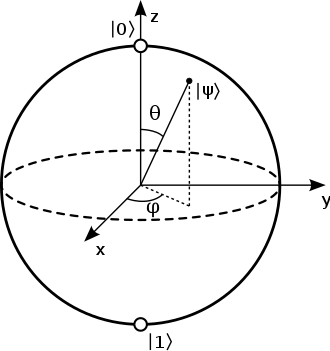
\includegraphics[scale=0.4]{img/330px-Bloch_sphere.png}
      \end{center}


      A few properties should be mentioned: 
      \begin{enumerate}
        \item The antiparallel vectors lying on the $X, Y, Z$ axes represent the orthonormal $X, Y, Z$ basis in $\mathbb{C}^2$. Note that while the basis is pairwise perpendicular in $\mathbb{C}^2$, in the Bloch sphere they are visualized as antiparallel. 

        \item The probability of it being $|0\rangle$ or $|1\rangle$ depends on the value of $\theta$. 
      \end{enumerate}
    \end{definition}

    



    The other kind of phase is known as the \textbf{relative phase factor}. Given two states

      \[|\psi \rangle = \alpha |0\rangle + \beta |1\rangle \text{ and } |\psi^* \rangle = \alpha^* |0 \rangle + | \beta^* \rangle,\]

    if $|\alpha| = |\alpha^*|$ or $|\beta| = |\beta^*|$, then we say that \textbf{the amplitudes differ by a relative phase}. Furthermore, two states $|\psi \rangle, |\psi^* \rangle$ are said to \textbf{differ by a relative phase in some basis} if each of the amplitudes in that basis is related by such a phase factor. For example, two states 

    \[\frac{|0\rangle + |1\rangle}{\sqrt{2}} \text{ and } \frac{|0\rangle - |1\rangle}{\sqrt{2}}\]
    differ by a relative phase (in the computational basis $|0\rangle, |1\rangle$) since the $|0\rangle$ amplitudes differ by a relative phase factor of $1$ ($ \frac{1}{\sqrt{2}} = 1 \cdot \frac{1}{\sqrt{2}}$) and the $|1\rangle$ amplitudes differ by a relative phase factor of $-1$ ($-\frac{1}{\sqrt{2}} = -1 \cdot \frac{1}{\sqrt{2}}$). It is clear that due to Born's rule on this one-qubit system, $|\alpha| = |\alpha^*| \iff |\beta| = |\beta^*|$, and so, all we have to do is check the magnitudes of the $|0\rangle$ amplitudes of two state vectors. Visualizing this on the Bloch sphere, we can see that the $\theta$ is the only parameter capable of changing the $|0\rangle$ amplitude. The global phase factor $e^{i\gamma}$ is merely a rotation map and also cannot change the $|0\rangle$. Therefore, we can see that two state vectors differ by a relative phase if and only if they have the same $\theta$ value, i.e. if the two points on the Bloch sphere are on the same "latitude."

    \begin{center} 
      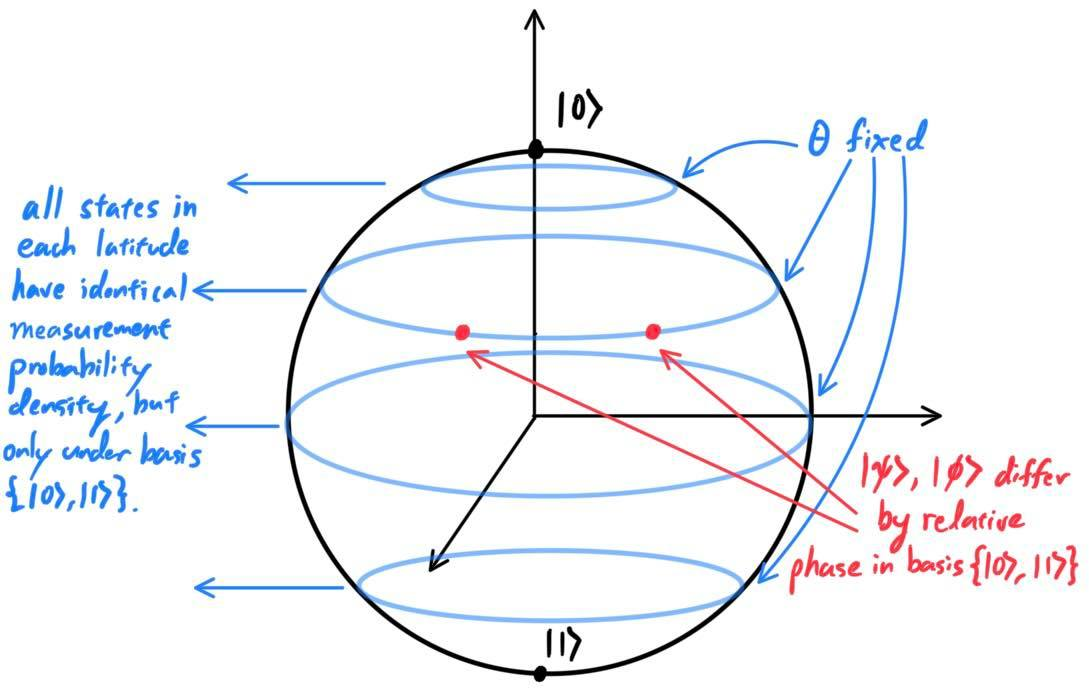
\includegraphics[scale=0.3]{img/Bloch_Sphere_latitude.jpg}
    \end{center}

    Notice that if two states are differ by a relative phase, then these phases are observationally equivalent, and so must be similar to the global phase factor. However, the relative phase is basis-dependent and so may produce different probability densities depending on the computational basis, while the global one is basis-independent. 

  \subsection{Entanglement}

    If we are interested in a composite quantum system made up of two (or more) distinct physical systems, the states of the composite system can be described as stated in postulate 4. 

    \begin{theorem}[Postulate 4: Composite Systems]
      The state space of a composite physical system is the tensor product of the state spaces of the component physical systems. That is, if we have systems $1, \ldots, n$ with the state vector of the $i$th system being $|\psi_i \rangle$, then the joint state of the total system is

        \[\bigotimes_i |\psi_i \rangle = |\psi_1 \rangle \otimes |\psi_2 \rangle \otimes \ldots \otimes |\psi_n \rangle.\]
    \end{theorem}

    A further property of the tensor product of Hilbert spaces is the induced inner product. That is, if $H_1$ and $H_2$ are Hilbert spaces with inner products $\langle \cdot, \cdot \rangle_1$ and $\langle \cdot, \cdot \rangle_2$, respectively, then $H_1 \otimes H_2$ is a Hilbert space with an induced inner product

      \[\langle v_1 \otimes v_2 , w_1 \otimes w_2 \rangle \equiv \langle v_1, w_1\rangle_1 \; \langle v_2, w_2 \rangle_2\]

    for $v_1, w_1 \in H_1, \; v_2, w_2 \in H_2$. 

    \begin{example}[Two-Qubit System]
      By applying postulate 4, a two-qubit system can be represented in tensor product notation. Let us have qubits $\psi_0 = \alpha_0 \, |0\rangle + \beta_0 \, |1\rangle$ and $\psi_1 = \alpha_1 \, |0\rangle + \beta_1 \, |1\rangle$. Then, the tensor product notation of the two qubits can be represented as

        \[|\psi_0 \psi_1 \rangle = \begin{pmatrix} \alpha_0 \\ \beta_0 \end{pmatrix} \otimes \begin{pmatrix} \alpha_1 \\ \beta_1 \end{pmatrix} = \begin{pmatrix} \alpha_0 \alpha_1 \\ \alpha_0 \beta_1 \\ \beta_0 \alpha_1 \\ \beta_0 \beta_1 \end{pmatrix},\]

      with the important property that

        \[|\alpha_0 \alpha_1|^2 + |\alpha_0 \beta_1|^2 + |\beta_0 \alpha_1|^2 + |\beta_0 \beta_1|^2 = 1,\]

      where

      \begin{align*}
        \mathbb{P}(\text{collapse to } |00\rangle) & = |\alpha_0 \alpha_1|^2, \\
        \mathbb{P}(\text{collapse to } |01\rangle) & = |\alpha_0 \beta_1|^2, \\
        \mathbb{P}(\text{collapse to } |10\rangle) & = |\beta_0 \alpha_1|^2, \\
        \mathbb{P}(\text{collapse to } |11\rangle) & = |\beta_0 \beta_1|^2.
      \end{align*}

      But since this tensor product space has the basis

      \[
        |00\rangle = \begin{pmatrix} 1 \\ 0 \end{pmatrix} \otimes \begin{pmatrix} 1 \\ 0 \end{pmatrix}, \; 
        |01\rangle = \begin{pmatrix} 1 \\ 0 \end{pmatrix} \otimes \begin{pmatrix} 0 \\ 1 \end{pmatrix}, \; 
        |10\rangle = \begin{pmatrix} 0 \\ 1 \end{pmatrix} \otimes \begin{pmatrix} 1 \\ 0 \end{pmatrix}, \; 
        |11\rangle = \begin{pmatrix} 0 \\ 1 \end{pmatrix} \otimes \begin{pmatrix} 0 \\ 1 \end{pmatrix}, 
      \]

      we can represent the two-qubit system more concisely as

        \[|\psi \rangle = \alpha_{00} |00\rangle + \alpha_{01} |01\rangle + \alpha_{10} |10\rangle + \alpha_{11} |11\rangle,\]

      with the measurement result $x ( = 00, 01, 10, 11)$ occurring with probability $|\alpha_{x}|^2$.
    \end{example}

    We can now talk about entanglement. 

    \begin{definition}[Entangled State]
      A state $|\psi\rangle$ of a composite system that cannot be written as the tensor product of the states of its component systems is said to be in an \textbf{entangled state}.   
    \end{definition}

    \begin{definition}[Bell States]
      The four maximally entangled states of two qubits are known as the \textbf{Bell states}. They are
      \begin{align}
        \ket{\Phi^+} & = \frac{|00\rangle + |11\rangle}{\sqrt{2}}, \\
        \ket{\Psi^+} & = \frac{|01\rangle + |10\rangle}{\sqrt{2}}, \\
        \ket{\Phi^-} & = \frac{|00\rangle - |11\rangle}{\sqrt{2}}, \\
        \ket{\Psi^-} & = \frac{|01\rangle - |10\rangle}{\sqrt{2}},
      \end{align}
      where the symbol represents the partity of the state ($\Phi$ for even and $\Psi$ for odd) and the exponent represents the relative phase of the state ($+$ for positive and $-$ for negative). 
    \end{definition}

    Note that the Bell states cannot be written down as the following product

    \begin{align*}
      \frac{|00\rangle + |11 \rangle}{\sqrt{2}} & \neq \big(\alpha |0\rangle + \beta |1\rangle \big) \otimes \big( \alpha^\prime |0 \rangle + \beta^\prime |1\rangle \big) \\
      & = \alpha \alpha^\prime |00\rangle + \alpha \beta^\prime |01\rangle + \beta \alpha^\prime |10\rangle + \beta \beta^\prime |11\rangle
    \end{align*}

    since this must mean that one of $\alpha$ or $\beta^\prime$ must be $0$. If $\alpha = 0$, then the $|00\rangle$ amplitude must be $0$ and if $\beta^\prime = 0$, then the $|11\rangle$ amplitude must be $0$, leading to a contradiction. 

    With further observation we can see that the majority of a composite Hilbert space consists of entangled states. That is, when we keep on adding qubits to the system, the total dimension grows as $2^n$. However, the number of states that can be written as a tensor product of the individual qubits is only $2n$. Therefore, the majority of the states in the composite Hilbert space are entangled. This is similar to how most probability distributions have correlation, i.e. are not factorable into a product of independent distributions. 

    \subsubsection{Bell's Inequality} 

      Neilsen and Chuwang pg 118 and before. 

  \subsection{Density Operators} 

    So far, we've been doing things given that we \textit{knew for sure what the state } $\ket{\psi}$ was. But what if we didn't know? We already had some uncertainty with measuring $\ket{\psi}$ with some observable, but now we have an additional layer of uncertainty on the state itself. This is where we can use density operators to represent \textit{mixed states}. 

    \begin{definition}[Density Operator]
      Let $i$ denote any set of index, and say that we have a quantum system in a state $\ket{\psi_i}$ with probability $p_i$. Then the \textbf{density operator} packages this ensemble of states into a single operator

        \[\rho = \sum_i p_i \ket{\psi_i} \bra{\psi_i}.\]

      If $|\{i\}| = 1$, then this is a \textbf{pure state}, and else it is a \textbf{mixed state}. 
    \end{definition}

    \begin{theorem}[Properties of Density Operators]
      The density operator has the following properties. 
      \begin{enumerate}
        \item It has unit trace: $\text{Tr}(\rho) = 1$.
        \item It is positive semidefinite: $\rho \geq 0$.
        \item It is self-adjoint: $\rho^\dagger = \rho$.
      \end{enumerate}
    \end{theorem}
    \begin{proof} 
      Listed. 
      \begin{enumerate} 
        \item By the cyclic trace property (just contraction of indices), we have 
          \begin{equation} 
            \text{Tr}(\rho) = \sum_i p_i \text{Tr}(\ket{\psi_i} \bra{\psi_i}) = \sum_i p_i \langle \psi_i | \psi_i \rangle = \sum_i p_i = 1.
          \end{equation}
        \item It is positive semidefinite since the eigendecomposition above shows that the eigenvalues are probabilities $p_i \geq 0$. 
        \item Again by the eigendecomposition, it is self-adjoint. 
      \end{enumerate}
    \end{proof}

    \begin{theorem}[Criterion to Decide if a State is Mixed or Pure]
      $\rho$ is pure if 
      \begin{enumerate} 
        \item $\mathrm{rank}(\rho) = 1$ 
        \item $\rho$ has $1$ eigenvalue equal to $1$, and rest equal to $0$, which implies that $\rho^2 = \rho$ (is a projection operator).
        \item $\mathrm{Tr}(\rho^2) = 1$ (since cyclic trace property). 
      \end{enumerate}

      $\rho$ is mixed if 
      \begin{enumerate} 
        \item $\mathrm{rank}(\rho) > 1$
        \item $\mathrm{Tr}(\rho) = \sum_i p_i^2 < 1$ (since $\rho^2 \neq \rho$).
      \end{enumerate}
    \end{theorem}

    We've basically restated the state space postulate in terms of density operators. Now we can talk about their evolution and measurements. Recall that given a pure state $\ket{\psi}$, evolution is given by a unitary operator $U$ acting on the state space. There is a natural extension for density operators. 

    \begin{lemma}[Evolution of Density Operators]
      Density operators evolve according to the rule 
      \begin{equation} 
        \rho \mapsto U \rho U^\dagger = \sum_i \rho_i U \ket{\psi_i} \bra{\psi_i} U^\dagger
      \end{equation}
      which makes sense since every $\ket{\psi}$ in the ensemble should also evolve unitarily according to $U$. 
    \end{lemma}

    When we conduct a projective measurement, we have a random variable representing what we observe $M$ and its associated Hamiltonian operator $\hat{M}$, the observable. We take the eigendecomposition of $\hat{M}$ into its projection matrices $\hat{P}_m$ that project onto the eigenvectors. The probability of observing outcome $m$ is 
    \begin{equation}
      \mathbb{P}(M = m) = \bra{\psi} \hat{P}_m \ket{\psi} 
    \end{equation}

    \begin{lemma}[Measurement of Density Operators]
      The above is really just like taking a trace of the $1 \times 1$ scalar generated, and so given a mixed state $\{ \ket{\psi_i}\}$, the measurement on the $i$th state of the ensemble is 
      \begin{equation}
        \mathbb{P}(M = m \mid i) = \mathrm{Tr}(\bra{\psi} \hat{P}_m \ket{\psi}) = \mathrm{Tr}( \hat{P}_m \ket{\psi_i} \bra{\psi_i}) 
      \end{equation}
      Using conditional probability and linearity, we can see that if we measure the mixed state $\rho$, the probability distribution of $M$ will be 
      \begin{equation}
        \mathbb{P}(M = m) = \sum_i \mathbb{P}(M = m \mid i) \mathbb{P}(i) = \sum_i \mathrm{Tr}(\hat{P}_m \ket{\psi_i} \bra{\psi_i}) \rho_i = \mathrm{Tr}(\hat{P}_m \rho) 
      \end{equation}
      After the measurement, we want to take each state in the ensemble, project it into $\hat{P}_m$, and then renormalize it. 
      \begin{equation}
        \rho \mapsto \rho^\prime = \sum_i \mathbb{P}(i \mid M = m) \frac{\hat{P}_m \ket{\psi_i} \bra{\psi_i} \hat{P_m}^\dagger}{\mathbb{P}(M = m \mid i)} \sum_i p(i) \frac{\hat{P}_m \ket{\psi_i} \bra{\psi_i} \hat{P}_m}{\mathbb{P}(M = m)} = \frac{\hat{P}_m \rho \hat{P}_m}{\mathrm{Tr}(\hat{P}_m \rho)} 
      \end{equation}
      Note that the trace of $\rho^\prime$ is still $1$. 
    \end{lemma}

    \begin{lemma}[Expectation of Measurements on Density Operators]
      Finally, the expectation value is simply 
      \begin{equation}
        \mathbb{E}(M) = \sum_m m \mathbb{P}(M = m) = \sum_m m \mathrm{Tr}(\hat{P}_m \rho) = \mathrm{Tr}(\hat{M} \rho)
      \end{equation}
    \end{lemma}

    Let us go through some examples of density operators. 

    \begin{example}[Simple Mixed State]
      Consider the qubits and their density operators: 
      \begin{align} 
        \ket{\psi} = \ket{0} & \implies \rho = \ket{0} \bra{0} \\
        \ket{\psi} = \ket{1} & \implies \rho = \ket{1} \bra{1} \\
        \ket{\psi} = \frac{1}{\sqrt{2}} ( \ket{0} + \ket{1}) & \implies \rho = \frac{1}{2} \big( \ket{0} \bra{0} + \ket{0} \bra{1} + \ket{1} \bra{0} + \ket{1} \bra{1} \big) 
      \end{align}
      These are all pure states,and by removing the middle two terms in the last operator, we can get a mixed state. 
      \begin{equation} 
        \rho = \frac{1}{2} \big( \ket{0} \bra{0} + \ket{1} \bra{1} \big) 
      \end{equation}
      which is a mixture $p_0 = p_1 = \frac{1}{2}$ of the pure states $\ket{0}$ and $\ket{1}$. 
    \end{example}

    \begin{exercise}
      Show that both of the pure state mixtures $\rho_1$ and $\rho_2$ in the previous exercise can be created from the 2 qubit maximally entangled Bell state $\ket{\Phi^+} = \frac{\ket{00} + \ket{11}}{\sqrt{2}}$ by projectively measuring one qubit and recombining the resulting single-qubit states into a single ensemble. 
      \begin{equation}
        \rho_1 = \rho_2 = \sum_k ( \bra{e_k} \otimes I_2) \rho_{\Phi} + (\ket{e_k} \otimes I_2)
      \end{equation}
      for $\ket{e_k}$ spanning two different measurement bases. 
    \end{exercise}

    \begin{exercise}
      Imagine you are given two ensembles of single-qubit quantum states, one pure $\ket{\psi} = \frac{\ket{0} + \ket{1}}{\sqrt{2}}$ and one mixed $\rho = \frac{1}{2} \ket{0} \bra{0} + \frac{1}{2} \ket{1} \bra{1}$. 
      \begin{enumerate}
        \item Describe an experimental protocol to distinguish between the two ensembles. 
        \item What is the minimum possible (best-case) number of measurements you would need to conclusively distinguish between the two ensembles? 
      \end{enumerate}
    \end{exercise}


    \subsubsection{Ensemble Equivalence}

      You can see that the density matrix is not necessarily unique from the example above. Therefore, we should not assume some unique ensemble of states behind this density operator, but rather an equivalence class of states. A natural question to ask is what class of ensembles give rise to a single density matrix? 

      \begin{definition}[Ensemble Equivalence]
        Two ensembles $\{p_i, \ket{\psi_i}\}$ and $\{q_i, \ket{\phi_i}\}$ are said to be \textbf{ensemble equivalent} if they give rise to the same density operator. 
        \begin{equation}
          \rho = \sum_i p_i \ket{\psi_i} \bra{\psi_i} = \sum_i q_i \ket{\phi_i} \bra{\phi_i}
        \end{equation}
      \end{definition}

      \begin{theorem}[Ensemble Equivalence]
        Let us have 2 ensembles $\{\ket{\psi_i}\}$ and $\{\ket{\phi_i}\}$ of size $M$ and $N$, respectively, with $M \leq N$. Then, the two ensembles are ensemble equivalent if the following holds: 
        \begin{enumerate}
          \item We first pad the smaller ensemble with $0$ vectors to make them the same size. 
          \item There exists a unitary operator $U$ such that $\ket{\phi_i} = U \ket{\psi_i}$
        \end{enumerate}
        Consequently, two ensembles $\{p_i, \ket{\psi_i}\} and \{q_i, \ket{\phi_i}\}$ have the same density matrix if and only if they are ensemble equivalent in the above sense and $U$ satisfies 
        \begin{equation}
          \sqrt{p_i} \ket{\psi_i} = \sum_j U_ij \sqrt{q_j} \ket{\phi_j}
        \end{equation}
      \end{theorem}
      \begin{proof}
        TBD, Neilsen and Chuwang pg 104. 
      \end{proof}

    \subsubsection{Pauli Decomposition of Density Operators}

      Recall the Pauli decomposition, which we can use to represent density operators. 

      \begin{definition}[Pauli Decomposition]
        The \textbf{Pauli Decomposition} is a generic decomposition for Hermitian $2 \times 2$ matrices. Since the Pauli matrices span the subspace of traceless Hermitian matrices, we can add in an identity to make the trace $1$. 
        \begin{equation}
          \rho(\mathbf{r}) = \frac{\mathbf{I} + \mathbf{r} \cdot \boldsymbol{\sigma}}{2}
        \end{equation}
        where the $\frac{1}{2}$ constant normalizes the trace. It is set to be the dimension of the underlying Hilbert space (i.e. $2$). 
      \end{definition}

      For pure states, we must have $\rho^2 = \rho$, and so 
      \begin{equation}
        \rho^2 = \frac{1}{4} \big( \mathbf{I} + 2 \mathbf{r} \cdot \boldsymbol{\sigma} + (\mathbf{r} \cdot \boldsymbol{\sigma})^2 \big)
      \end{equation}
      which is true if $||\mathbf{r}|| = 1$. This means that $\mathbf{r}$ must live on the unit sphere, i.e. the Bloch sphere. 

      \begin{example}[Pauli Decomposition of $\ket{0}$]
        If we have the pure state $\ket{\psi} = \ket{0}$, then 
        \begin{equation}
          \rho = \begin{pmatrix} 1 & 0 \\ 0 & 0 \end{pmatrix} \implies \mathbf{r} = \bigg( \frac{\mathrm{Tr}(X \rho)}{2}, \frac{\mathrm{Tr}(Y \rho)}{2}, \frac{\mathrm{Tr}(Z \rho)}{2} \bigg) = (0, 0, 1)
        \end{equation}
        If we have $\ket{\psi} = \ket{+}$, then 
        \begin{equation}
        \rho = \frac{1}{2} \begin{pmatrix} 1 & 1 \\ 1 & 1 \end{pmatrix} \implies \mathbf{r} = (1, 0, 0)
        \end{equation}
      \end{example}

      For mixed states, we must have $\rho^2 < \rho$ (as in the $\rho - \rho^2$ is positive semidefinite), so some algebra reveals that 
      \begin{equation}
        ||\mathbf{r}|| < 1
      \end{equation}
      and so $\mathbf{r}$ must live inside the Bloch sphere.

      \begin{example}[Pauli Decomposition of Maximally Mixed State]
        Given the ensembles $\{\ket{0}, \ket{1}\}$ or $\{\ket{+}, \ket{-}\}$, the density operator is 
        \begin{equation}
          \rho = \frac{1}{2} \begin{pmatrix} 1 & 0 \\ 0 & 1 \end{pmatrix}
        \end{equation}
        which we can see that $\mathbf{r} = (0, 0, 0)$, and so it is the center of the Bloch sphere. 
      \end{example}

    \subsubsection{Reduced Density Operator}
      
      We can also use the density operator to describe subsystems of a composite quantum system. To do this, we define the partial trace. 

      \begin{definition}[Partial Trace]
        Given a composite system on Hilbert space $V \otimes W$ and a linear map $A \otimes B: V \otimes W \rightarrow V \otimes W$, the \textbf{partial trace} of $A \otimes B$ is 
        \begin{equation}
          \mathrm{Tr}_B (A \otimes B) = A \cdot \mathrm{Tr}(B)
        \end{equation}
        which is just a tensor contraction over $B$. That is, by letting 
        \begin{equation}
          B = \sum_{i, j} \beta_{ij} e_i \otimes e_j \implies \mathrm{Tr}(B) = \sum_{i, j} \beta_{ij} e_i (e_j) = \sum_i \beta_{ii}
        \end{equation}
      \end{definition}

      \begin{definition}[Reduced Density Operator]
        The \textbf{reduced density operator} of a composite system is the partial trace of the density operator of the composite system. 
      \end{definition}

\section{Quantum Circuits}

    By solving the time-independent Schrodinger's equation, we have found out that closed quantum systems evolve according to a unitary operator. A question to ask is what kind of unitary operators are natural to consider? In the case of single qubits, it turns out that \textit{any} unitary operator at all can be realized in physical systems. Therefore, we can modify these qubits with general unitary operators, which are in some way a generalization of classical logic gates. Quantum logic gates can be interpreted as matrices that modify the state of qubits. 

    This is similar to those of classical gates, but one key difference between quantum logic gates and classical ones is that quantum gates are always invertible (from the unitary condition), while some classical gates like NAND are irreversible (e.g., if the output of a NAND gate is $1$, we don't know if the input is $00, 01$, or $10$). We can divide them into classes depending on how many arguments they take, but as we will see, the general form of a quantum gate taking in $n$ input qubits is some unitary matrix in $U(2^n)$. Let us first focus on gates of one qubit. We will start with the Pauli matrices and spend some time investigating their properties.  

    \begin{enumerate} 
      \item Quantum circuits are acyclic, meaning that there are no loops, unlike classical circuits. 
      \item Classical circuits have the bits either being $\ket{0}$ or $\ket{1}$. Quantum circuits have the qubits being in a superposition $\ket{\psi} = \alpha \ket{0} + \beta \ket{1}$. 
      \item Classical circuits allow wires to be joined together (e.g. FANIN) or split/copied (e.g. FANOUT). Quantum circuits cannot do this since it is not invertible. Every gate must be a $n \times n$ unitary operator.
    \end{enumerate}
    
    It is common to use both classical bits and qubits in a quantum circuit. To distinguish between the two, we use two lines to denote the flow of classical bits and a single line to denote the flow of qubits. This is clarified in the following examples. 

  \subsection{Classical Logic Gates} 

    Before we begin with quantum circuits, it is good to draw analogies to classical circuits. Recall the following below, with notation changed to quantum mechanical notation. 

    \begin{definition}[Classical NOT]
      The not gate is 
    \end{definition}

    \begin{definition}[Classical AND]
      
    \end{definition}

    \begin{definition}[Classical XOR]
      In the general case, the XOR gate maps
      \begin{equation} 
        \text{XOR}: \; (A, B) \mapsto (A, A \oplus B)
      \end{equation}
      where $A$ and $B$ are classical bits. This can be used as a FANOUT gate, and so we can use it to copy a bit. 
    \end{definition}

  \subsection{Quantum Logic Gates}

    \begin{definition}[Pauli X]
      The Pauli X gate is the quantum equivalent of the classical NOT gate. 
      \begin{enumerate} 
        \item It transforms as such: 
          \begin{equation} 
            \alpha \ket{0} + \beta \ket{1} \mapsto \beta \ket{0} + \alpha \ket{1}
          \end{equation}
        \item with the matrix form: 
          \begin{equation} 
            \begin{pmatrix} 0 & 1 \\ 1 & 0 \end{pmatrix}
          \end{equation}
        \item and the circuit form: 
          \begin{center}
            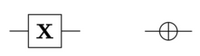
\includegraphics[scale=0.5]{img/Pauli_X_gate.png}
          \end{center}
        \item It also flips the state of the qubit in the Bloch sphere about the $X$-axis. 
      \end{enumerate}
    \end{definition}

    \begin{definition}[Pauli Y]
      The Pauli Y gate 
      \begin{enumerate} 
        \item It transforms as such: 
          \begin{equation} 
            \alpha \ket{0} + \beta \ket{1} \mapsto  i \beta \ket{0} - i \alpha \ket{1}
          \end{equation}
        \item with the matrix form: 
          \begin{equation} 
            \begin{pmatrix} 0 & -i \\ i & 0 \end{pmatrix}
          \end{equation}
        \item and the circuit form: 
          \begin{center}
            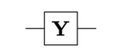
\includegraphics[scale=0.5]{img/Pauli_Y_gate.png}
          \end{center}
        \item It also flips the state of the qubit in the Bloch sphere about the $Y$-axis. 
      \end{enumerate}
    \end{definition}

    \begin{definition}[Pauli Z]
      The Pauli Z gate simply flips the sign of the coefficient of $\ket{1}$. 
      \begin{enumerate} 
        \item It transforms as such: 
          \begin{equation} 
            \alpha \ket{0} + \beta \ket{1} \mapsto \alpha \ket{0} - \beta \ket{1}
          \end{equation}
        \item with the matrix form: 
          \begin{equation} 
            \begin{pmatrix} 1 & 0 \\ 0 & -1 \end{pmatrix}
          \end{equation}
        \item and the circuit form: 
          \begin{center}
            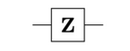
\includegraphics[scale=0.5]{img/Pauli_Z_gate.png}
          \end{center}
        \item It also flips the state of the qubit in the Bloch sphere about the $Z$-axis. 
      \end{enumerate}
    \end{definition}

    Since the Pauli matrices form a basis for the space of $2 \times 2$ Hermitian matrices, any unitary operator acting on a single qubit can be written as a linear combination of the Pauli matrices. By setting $\boldsymbol{\sigma} = (\sigma_1, \sigma_2, \sigma_3)$ to be the vector of Pauli matrices, we can write any unitary operator as 
    \begin{equation}
       \mathbf{v} \cdot \boldsymbol{\sigma} = v_1 \sigma_1 + v_2 \sigma_2 + v_3 \sigma_3
    \end{equation}

    \begin{definition}[Hadamard]
      The \textbf{Hadamard gate} $H$ takes in $|0\rangle$ or $|1\rangle$ and puts it into exactly equal superposition. That is, $H|0\rangle = |+\rangle$ and $H|1\rangle = |-\rangle$. Furthermore, it can take Bell states and put them into either $\ket{0}$ or $\ket{1}$. 
      \begin{enumerate} 
        \item It transforms as such: 
          \begin{equation} 
            \alpha \ket{0} + \beta \ket{1} \mapsto \frac{\alpha + \beta}{\sqrt{2}} \ket{0} + \frac{\alpha - \beta}{\sqrt{2}} \ket{1}
          \end{equation}
        \item with the matrix form 
          \begin{equation} 
            H = \frac{1}{\sqrt{2}} \begin{pmatrix} 1 & 1 \\ 1 & -1 \end{pmatrix}
          \end{equation}
        \item and the circuit form 
          \begin{center}
            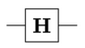
\includegraphics[scale=0.5]{img/Hadamard_gate.png}
          \end{center}
        \item This can be thought of as a rotation around the Bloch vector $(1, 0, 1)$.
      \end{enumerate}
    \end{definition}

    The next set consists of multiple qubit gates. Recall that any function of bits can be computed from the composition of NAND gates alone, which is known as a \textbf{universal gate}. The multi-qubit universal quantum gate is actually the control-not gate.

    \begin{definition}[Swap]
      The \textbf{swap} gate simply swaps the states of the two qubits.
      \begin{enumerate} 
        \item It transforms as such: 
          \begin{equation} 
            a |00\rangle + b |01\rangle + c|10\rangle + d|11\rangle \mapsto a |00\rangle + c |01\rangle + b|10\rangle + d|11\rangle
          \end{equation}
        \item with the matrix form 
          \begin{equation} 
            U_{SWAP} = \begin{pmatrix} 1&0&0&0\\0&0&1&0\\0&1&0&0\\0&0&0&1 \end{pmatrix}
          \end{equation}
        \item and the circuit form 
          \begin{center}
            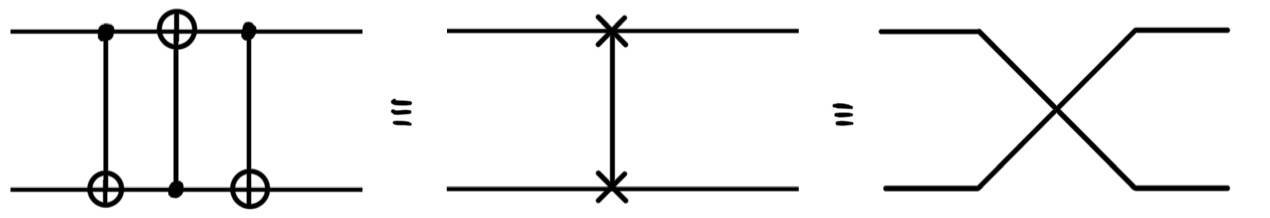
\includegraphics[scale=0.3]{img/Swap_Gate.jpg}
          \end{center}
      \end{enumerate}
    \end{definition}

    \begin{definition}[Control NOT]
      The \textbf{controlled-NOT} is a 2 qubit gate that has a control qubit. If the control qubit is set to $|0\rangle$, then the target qubit is left alone. If the control qubit is set to $|1\rangle$, then the target qubit is flipped. This seems a bit confusing since a qubit can be neither $\ket{0}$ nor $\ket{1}$, but this rule applies to each component of the tensor product. 
      \begin{enumerate} 
        \item It transforms as such: 
          \begin{equation} 
            a |00\rangle + b |01\rangle + c|10\rangle + d|11\rangle \mapsto a |00\rangle + b |01\rangle + d|10\rangle + c|11\rangle
          \end{equation}
        \item with the matrix form: 
          \begin{equation} 
            U_{CNOT} = \begin{pmatrix} I & 0 \\ 0 & X \end{pmatrix} = \begin{pmatrix} 1&0&0&0\\0&1&0&0\\0&0&0&1\\0&0&1&0 \end{pmatrix}
          \end{equation}
        \item and the circuit form
          \begin{center}
            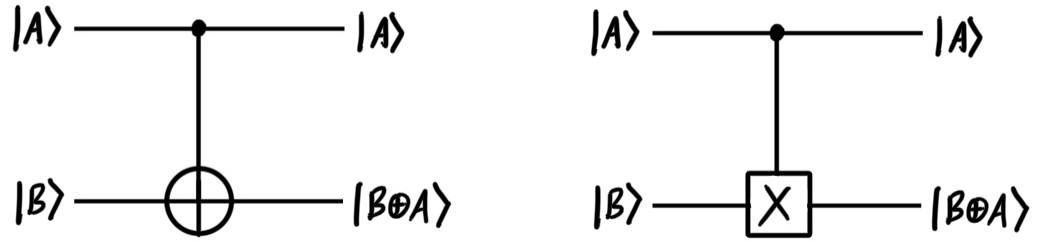
\includegraphics[scale=0.3]{img/Control_Not_gate.jpg}
          \end{center}
      \end{enumerate} 
      Notice how unlike the swap gate, the output 4-vector of the CNOT gate is not always guaranteed to decompose into a tensor product $|\psi_1 \rangle \otimes |\psi_2 \rangle$ of vectors (more on Bell states later). Its circuit is represented in the given image.
    \end{definition}

    At this point, we can now consider an extremely useful application: generating entangled states. Essentially, given two qubits $\ket{00}$, we can use a Hadamard gate to put the first qubit into a superposition, and then use a CNOT gate to introduce some correlation, ultimately entangling the two qubits. 

    \begin{lemma}[Entangling Qubits]
      Given a two qubit system, we can use a Hadamard gate and a CNOT gate to entangle the two qubits as such: 
      \begin{enumerate} 
        \item Apply a Hadamard gate to the first qubit. 
        \item Apply a CNOT gate with the first qubit as the control and the second qubit as the target.
      \end{enumerate}
      By doing this produre to the four computational basis states $\ket{00}, \ket{01}, \ket{10}, \ket{11}$, can get get all four Bell states. 
      \begin{figure}[H]
        \centering 
        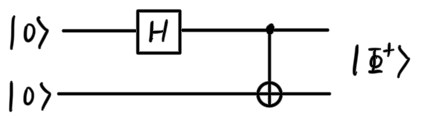
\includegraphics[scale=0.5]{img/Entangling_qubits.png}
        \caption{Entangling procedure done for the $\ket{00}$ basis state to produce $\ket{\Phi^+}$. } 
        \label{fig:entangling_qubits}
      \end{figure}
      Furthermore, we can just start off with the $\ket{00}$ state and apply some unitary gate $U$ on the first qubit to get all 4 Bell states. 
      \begin{figure}[H]
        \centering 
        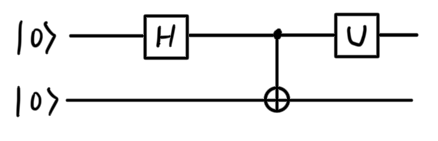
\includegraphics[scale=0.4]{img/Entangling_qubits_with_U.png}
        \caption{Entangling procedure done for the $\ket{00}$ basis state to produce any of the 4 Bell states. Setting $U =I, X, Z, ZX$ gives the bell states $\ket{\Phi^+}, \ket{\Psi^+}, \ket{\Phi^-}, \ket{\Psi^-}$.}
        \label{fig:entangling_qubits_with_U}
      \end{figure}
    \end{lemma}

    \begin{definition}[Control U]
      The \textbf{controlled-U} gate is a generalization of controlled-NOT. Let us have a control bit and $n$ target bits. If the control bit is set to $|0 \rangle$, then the target qubits are left alone. If the control qubit is set to $|1\rangle$, then the states/spins of the $n$ target qubits are changed by some unitary matrix $U \in \text{U}(2^n)$.
      \begin{enumerate} 
        \item It transforms as such: 
          \begin{equation} 
            a \ket{0} \otimes \ket{\psi} + b \ket{1} \otimes \ket{\psi} \mapsto a \ket{0} \otimes \ket{\psi} + b \ket{1} \otimes U \ket{\psi}
          \end{equation}
        \item with the matrix form: 
          \begin{equation} 
            U_{CU} = \begin{pmatrix} I & 0 \\ 0 & U \end{pmatrix}
          \end{equation}
        \item and the circuit form: 
          \begin{center}
            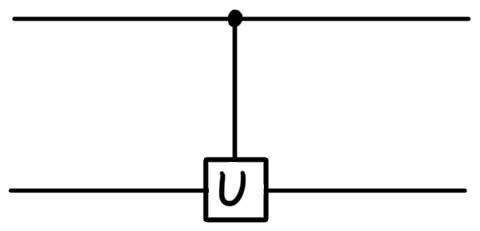
\includegraphics[scale=0.3]{img/Control_U_gate.jpg}
          \end{center}
      \end{enumerate}
    \end{definition}

    \begin{definition}[Toffoli]
      The \textbf{Toffoli} gate is similar to a CNOT but with two control qubits and 1 target qubit. If the control qubits are set to $|11\rangle$, then the target qubit is flipped.
      \begin{enumerate} 
        \item It transforms as such: 
          \begin{align*}
            a|000\rangle & + b|001\rangle + c|010\rangle + d |011\rangle + e|100\rangle + f |101\rangle + g|110\rangle + h|111\rangle \\
            \mapsto & a|000\rangle + b|001\rangle + c|010\rangle + d |011\rangle + e|100\rangle + f |101\rangle + h|110\rangle + g|111\rangle.
          \end{align*}
        \item with the matrix form: 
          \begin{equation} 
            T = \begin{pmatrix} 1&0&0&0&0&0&0&0\\ 0&1&0&0&0&0&0&0\\ 0&0&1&0&0&0&0&0\\ 0&0&0&1&0&0&0&0\\ 0&0&0&0&1&0&0&0\\ 0&0&0&0&0&1&0&0\\ 0&0&0&0&0&0&0&1\\ 0&0&0&0&0&0&1&0 \end{pmatrix}
          \end{equation}
        \item and the circuit form: 
          \begin{center}
            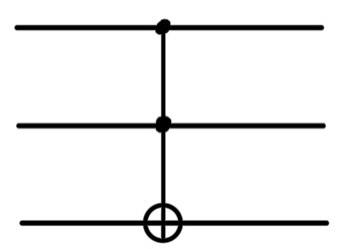
\includegraphics[scale=0.3]{img/Toffoli_gate.jpg}
          \end{center}
      \end{enumerate}
    \end{definition}
    
    At this point, we can see that we can have an arbitrary number of qubits which act as a control for some unitary operator. This gives us great flexibility in constructing quantum circuits.

    \begin{definition}[Measurement]
      Finally, we introduce the operation of "measurement," which we represent by a meter symbol.
      \begin{center}
        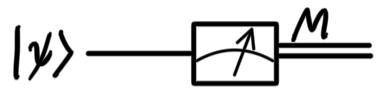
\includegraphics[scale=0.3]{img/Measurement_gate.jpg}
      \end{center}
      This operation converts a single qubit state $| \psi \rangle = \alpha |0\rangle + \beta |1\rangle$ into a probabilistic classical bit $M$, which is $0$ with probability $|\alpha|^2$ or $1$ with probability $|\beta|^2$. 
    \end{definition}

  \subsection{Physical Implementation} 

\section{Quantum Computation and Properties}

  \subsection{Quantum Tomography}

    In quantum computing, uncertainty is a huge obstacle to overcome, and it is not always the case that we know which state we are working with in a qubit. In a classical computer, we can always measure the state of a bit\footnote{You can simply measure the electrical pulse going through a wire. Presence indicates that it is turned on, a $1$, and the absence indicates that it is off, a $0$. } However, this is much harder in quantum computing. It is not so simple to just ``see'' which state a qubit is in, but it is possible. We typically do this through measurements, but as we know, measurements collapse the state of the qubit. Therefore, we want to measure some qubit (or an ensemble of identical qubits) and then reconstruct the state of the qubit according to the information that we have gained from our qubits. 

    \begin{definition}[Quantum Tomography]
      \textbf{Quantum tomography} refers to the process of determining the state of some system by measuring a system of identical systems. That is, while measurements tell you the state of the system after the measurement, tomography gives you insight about what the state was \textit{before} the measurement. Then, with this system we can reconstruct the state of the qubit.\footnote{This can be done by constructing the correct gate $G$ and just putting a bunch of $\ket{0}$ states through it.}
    \end{definition}

    In the end, it is just a question of \textit{what is the maximal amount of information I can extract from this system to reconstruct it?}. Sometimes, this is not possible to know for certain, but we can say with high probability. This is very similar to the problem of statistics, and in a way it is. We essentially have some distribution, and every measurement samples from that distribution. Given these samples, we want to reconstruct the distribution, and techniques like maximum likelihood or Bayesian updating are even used. But let's not get ahead of ourselves and start with an example. There are many assumptions that get thrown around, listed below, and we should know the basic ones. 

    \begin{enumerate}
      \item Whether we are trying to determine the state of a single qubit or a system of multiple qubits. 
      \item Whether we know a set of state $\{\ket{\psi_i}\}$ that the true state is in. 
      \item Whether these states are orthonormal. 
      \item How many qubits are prepared for us to work with?\footnote{Note that this must be finite, since if it was infinite, then we can measure with infinite precision and our state is trivially constructed.}
    \end{enumerate}

    \begin{example}[Distinguishing Two Orthonormal States]
      You are given a single qubit $\ket{\psi}$ which can be in one of two orthonormal state $\ket{\psi_1}$ and $\ket{\psi_2}$. It turns out that you can perfectly distinguish these states. 
      \begin{enumerate}
        \item Construct a measurement operator 
          \begin{equation}
            \hat{M} = 1 \cdot \hat{P}_1 + 2 \cdot \hat{P}_2 = 1 \cdot \ket{\psi_1} \bra{\psi_1} + 2 \cdot \ket{\psi_2} \bra{\psi_2} 
          \end{equation}
        \item When you measure the qubit $\ket{\psi}$, it must be an eigenvector of $\hat{M}$. Let $p$ be the random variable of the prepared state. Then 
          \begin{align}
            \mathbb{P}(M = 1 \mid p = \ket{\psi_1}) & = \bra{\psi_1} \hat{P}_1 \ket{\psi_1} = 1 \\ 
            \mathbb{P}(M = 1 \mid p = \ket{\psi_2}) & = \bra{\psi_2} \hat{P}_1 \ket{\psi_2} = 0 \\ 
            \mathbb{P}(M = 2 \mid p = \ket{\psi_1}) & = \bra{\psi_1} \hat{P}_2 \ket{\psi_1} = 0 \\
            \mathbb{P}(M = 2 \mid p = \ket{\psi_2}) & = \bra{\psi_2} \hat{P}_2 \ket{\psi_2} = 1
          \end{align}

        \item Therefore, if you observe $M = 1$, then it must have been the case that the state was $\ket{\psi_1}$, and if you observe $M = 2$, then it must have been the case that the state was $\ket{\psi_2}$. To formalize this, it is just simply Bayes rule. 
          \begin{align}
            \mathbb{P}(p = \ket{\psi_1} \mid M = 1) & = \frac{\mathbb{P}(M = 1 \mid p = \ket{\psi_1}) \mathbb{P}(p = \ket{\psi_1})}{\mathbb{P}(M = 1)} = 1 \\
            \mathbb{P}(p = \ket{\psi_2} \mid M = 2) & = \frac{\mathbb{P}(M = 2 \mid p = \ket{\psi_2}) \mathbb{P}(p = \ket{\psi_2})}{\mathbb{P}(M = 2)} = 1
          \end{align}
      \end{enumerate}
    \end{example}

    We can see that depending on what the measurement outcome realizes to, there is a probability of us being certain of the state. Let's define this metric. 

    \begin{definition}[Probability of Certainty]
      The \textbf{probability of certainty} is the probability of some measurement outcome $M$ being realized that gives us certainty of the state. 
    \end{definition}

    Therefore, the probability of certainty of the example above was $1$. Okay, that was easy, but what if the states were not orthonormal? It turns out that it is impossible to perfectly distinguish between two non-orthonormal states, even if we have an unbounded but finite number of identically prepared states to work with. 

    \begin{lemma}[Distinguishing Non-Orthonormal States]
      Given a finite number of $n$ qubits identically prepared at state $\ket{\psi}$ which can take states within the set $\{ \ket{\psi_i}\}$, it is not possible to perfectly distinguish them if the states are not orthonormal. 
    \end{lemma}
    \begin{proof}
      Suppose it is possible, corresponding to the measurement $M$ with its Hermitian operator $\hat{M}$. Then, it should be the case that if we start with state $\ket{\psi_1}$, then $\mathbb{P}(M = 1) = 1$, meaning that $\ket{\psi_1}$ must be an eigenvector of $M$. This holds true for $\ket{\psi_2}$ and so it must also be an eigenvector. However, this violates the contrapositive of the Spectral theorem which states that \textit{if $A$ is Hermitian on $V$, then there exists an orthonormal basis of $V$ consisting of eigenvectors of $A$}. 
    \end{proof}

    We can still distinguish them with high probability the more prepared states we have, but before blindly doing this, we should try to maximally optimize each measurement. Note that there are three stages to this process: 
    \begin{enumerate}
      \item Prepare the state $\ket{\psi}$. 
      \item Measure the state $\ket{\psi}$ with some measurement operator $\hat{M}$. 
      \item Guess the state $\ket{\psi}$ based on the measurement outcome. 
    \end{enumerate}
    The user can control the measurement operator and separately determine a strategy for guessing the state. We have implicitly made a strategy above using basic probability, but you can make completely bogus strategies even if you have the optimal measurement operator. With this in mind, we define more fine metrics. 

    \begin{definition}[(Maximal) Probability of Success]
      Given some measurement operator $\hat{M}$ and some strategy $\mathcal{S}$, the \textbf{probability of success} is the probability that the strategy $\mathcal{S}$ correctly guesses the state $\ket{\psi}$ given the measurement outcome $M$. The \textbf{maximal probability of success} is the maximum probability of success over all strategies. Note that for such thing to exist we must place a prior distribution over the states (i.e. know the probability of each state being prepared). 
    \end{definition}

    \begin{example}[Distinguishing Two Non-Orthonormal States]
      Suppose we have a single $\ket{\psi}$ qubit which can be in one of two states $\ket{\psi_1} = \ket{0}$ and $\ket{\psi_2} = \ket{+} = \frac{\ket{0} + \ket{1}}{\sqrt{2}}$, prepared with equal probability. We can naively construct the measurement operator 
      \begin{equation}
        \hat{M} = 1 \cdot \hat{P}_1 + 2 \cdot \hat{P}_2 = 1 \cdot \ket{0} \bra{0} + 2 \cdot \ket{1} \bra{1}
      \end{equation} 
      By focusing on $\ket{0}$ and setting the other one to be $\ket{0^\perp}$. We know this won't be perfect, but hopefully it will give us a decent chance of predicting correctly. We want to calculate both the probability of certainty and the maximal probability of success. First, let's compute some probabilities. 
      \begin{align}
        \mathbb{P}(M = 1 \mid p = \ket{0}) & = \bra{0} \hat{P}_1 \ket{0} = 1 \\ 
        \mathbb{P}(M = 1 \mid p = \ket{+}) & = \bra{+} \hat{P}_1 \ket{+} = \frac{1}{2} \\ 
        \mathbb{P}(M = 2 \mid p = \ket{0}) & = \bra{0} \hat{P}_2 \ket{0} = 0 \\ 
        \mathbb{P}(M = 2 \mid p = \ket{+}) & = \bra{+} \hat{P}_2 \ket{+} = \frac{1}{2} 
      \end{align}
      Therefore, with Bayes rule, we can compute 
      \begin{align}
        \mathbb{P}(p = \ket{0} \mid M = 1) & = \frac{2}{3} \\ 
        \mathbb{P}(p = \ket{+} \mid M = 1) & = \frac{1}{3} \\ 
        \mathbb{P}(p = \ket{0} \mid M = 2) & = 0 \\ 
        \mathbb{P}(p = \ket{+} \mid M = 2) & = 1
      \end{align}
      and the probability of certainty is 
      \begin{align}
        \mathbb{P}(M = 2) & = \mathbb{P}(M = 2 \mid p = \ket{0}) \mathbb{P}(p = \ket{0}) + \mathbb{P}(M = 2 \mid p = \ket{1}) \mathbb{P}(p = \ket{1}) \\
                          & = 0 \cdot \frac{1}{2} + \frac{1}{2} \cdot \frac{1}{2} = \frac{1}{4}
      \end{align}
      With this measurement operator, our optimal strategy would be to just simply choose the state with the maximal probability in the posterior. If $M = 1$, we should choose $\ket{0}$ and if $M = 2$, we should choose $\ket{+}$. The maximal probability of success is 
      \begin{equation}
        \mathbb{P}(M = 1 \mid p = \ket{0}) \mathbb{P}(p = \ket{0}) + \mathbb{P}(M = 2 \mid p = \ket{+}) \mathbb{P}(p = \ket{+}) = \frac{1}{2} \cdot \frac{1}{2} + 1 \cdot \frac{1}{2} = \frac{3}{4}
      \end{equation}
    \end{example}

    Determining the best strategy is pretty easy, but what about the best operator? Well this is simply just an optimization problem. 

    \begin{example}[Best Operator for Distinguishing Two Non-Orthonormal States]
      Given the same situation above, let's be a bit smarter about constructing $\hat{M}$. It must be defined over some orthonormal basis, so we can parameterize it from the Bloch sphere: 
      \begin{align}
        \ket{\psi} & = \cos\frac{\theta}{2} \ket{0} + e^{i \phi} \sin\frac{\theta}{2} \ket{1} \\
        \ket{\psi^\perp} & = e^{-i \phi} \sin\frac{\theta}{2} \ket{0} - \cos\frac{\theta}{2} \ket{1}
      \end{align}
      and so our measurement is 
      \begin{equation}
        \hat{M} = 1 \cdot \hat{P}_1 + 2 \cdot \hat{P}_2 = 1 \cdot \ket{\psi} \bra{\psi} + 2 \cdot \ket{\psi^\perp} \bra{\psi^\perp}
      \end{equation}
      Therefore, we can compute with some trigonometric identities 
      \begin{align}
        \mathbb{P}(M = 1 \mid p = \ket{0}) & = \bra{0} \hat{P}_1 \ket{0} = \cos^2 \frac{\theta}{2} \\ 
        \mathbb{P}(M = 1 \mid p = \ket{+}) & = \bra{+} \hat{P}_1 \ket{+} = \frac{1}{2} + \frac{1}{2} \sin{\theta} \cos{\phi} \\ 
        \mathbb{P}(M = 2 \mid p = \ket{0}) & = \bra{0} \hat{P}_2 \ket{0} = \sin^2 \frac{\theta}{2} \\ 
        \mathbb{P}(M = 2 \mid p = \ket{+}) & = \bra{+} \hat{P}_2 \ket{+} = \frac{1}{2} - \frac{1}{2} \sin{\theta} \cos{\phi}
      \end{align}
      Notice that computing the inverse conditionals with Bayes rule isn't necessary. These probabilities are only required for us to compute the probability of certainty, but we know that as long as the optimal basis does not coincide with the possible states, this will be $0$. Let's directly go into calculating the maximal probability of success, which is 
      \begin{align}
        \mathbb{P}(\text{success}) & = \mathbb{P}(M = 1 \mid p = \ket{0}) \mathbb{P}(p = \ket{0}) + \mathbb{P}(M = 2 \mid p = \ket{+}) \mathbb{P}(p = \ket{+}) \\
                                   & = \cos^2 \frac{\theta}{2} \cdot \frac{1}{2} + \bigg( \frac{1}{2} - \frac{1}{2} \sin{\theta} \cos{\phi} \bigg) \cdot \frac{1}{2}
      \end{align}
      We want to maximize this, and first we can remove all the constant terms. Second, we can see that maximizing w.r.t. $\phi$ is independent of $\theta$, and so we can set $\phi = 0$. Then, we can maximize w.r.t. $\theta$ to get the maximal probability of success. We just set the derivative to $0$ and solve. 
      \begin{equation}
        0 = \frac{d}{d\theta} \bigg\{ \cos^2 \frac{\theta}{2} - \frac{1}{2} \sin{\theta} \bigg\} \implies  \theta = \frac{\pi}{4}
      \end{equation}
      Therefore, our optimal measurement basis is 
      \begin{equation}
        \ket{\psi} = \cos\frac{\pi}{8} \ket{0} + \sin\frac{\pi}{8} \ket{1} 
      \end{equation}
      and our maximal probability of success is 
      \begin{equation}
        \mathbb{P}(\text{success}) = \frac{1}{2} + \frac{1}{2 \sqrt{2}}
      \end{equation}
    \end{example}

    Geometric interpretation. 

    \begin{theorem}[]
      The maximum probability of success to distinguish two states $\ket{\psi_1}, \ket{\psi_2}$ is 
      \begin{equation}
        \mathbb{P}(\text{success}) = \frac{1 + \sin(\arccos(|\braket{\psi_1}{\psi_2}|))}{2}
      \end{equation}
    \end{theorem}

    \begin{theorem}[Holevo Bound]
      The Holevo bound is a generalization of the previous theorem to $n$ states. 
      \begin{equation}
        \mathbb{P}(\text{success}) \leq 1 - H\bigg( \frac{1 + |\braket{\psi_1}{\psi_2}|}{2} \bigg)
      \end{equation}
      where $H$ is the binary entropy function.
    \end{theorem}

  \subsection{Parity Operators}

    Quantum tomography is the first tool we need to work with states, but we have said that often we need an ensemble of identical qubits to work with so we can make an optimal series of measurements. This is needed since these measurements are destructive, and we need to make sure that we can extract as much information as possible. But every measurement does not necessarily have to be destructive. We can use \textit{partial projective measurements} to extract information while still keeping it in some superposition by projecting the system into some non-degenerate eigenspace of our measurement operator $\hat{M}$. 

    \begin{example}[Computing Parity]
      Say that we have a $n$-qubit state $\ket{\psi}$ and we want to measure the parity of the state. There are two ways that we can do this: 
      \begin{enumerate}
        \item We can perform a complete Von Neumann measurement with respect to the computational basis and subsequently compute the parity of the resulting string. 
        \item We can perform a projective measurement of the parity with the operator $Z^{\otimes n}$ 
      \end{enumerate}
      They both measure the parity of the realized system, but the difference is what the system collapses to. Let's have a state $\ket{\psi} = \alpha_{00} \ket{00} + \alpha_{01} \ket{01} + \alpha_{10} \ket{10} + \alpha_{11} \ket{11}$. Then, I can take an ancilla qubit in the state $\ket{0}$ and conduct the parity measurement 
      \begin{equation}
        U_p = (\ket{00} \bra{00} + \ket{11} \bra{11}) \otimes I + (\ket{01} \bra{01} + \ket{10} \bra{10}) \otimes X
      \end{equation}
      which brings the state to 
      \begin{equation} 
        \ket{\psi} \otimes \ket{0} \xrightarrow{U_p} (\alpha_{00} \ket{00} + \alpha_{11} \ket{11}) \otimes \ket{0} + (\alpha_{01} \ket{01} + \alpha_{10} \ket{10}) \otimes \ket{1}
      \end{equation}
      By conducting a partial projective measurement on the third qubit, we are essentially projecting the state to the eigenspace corresponding to the parity of the state, which is spanned by either $\{\ket{00} + \ket{11}\}$ and $\{\ket{01} + \ket{10}\}$. Therefore, the second measurement may be preferred since we can directly observe parity without destroying the superposition of the system.
    \end{example}

    We can get a good geometric interpretation of this. Initially, there is some quantum system $\ket{\psi}$ in some Hilbert space $\mathcal{H}$. Every projective measurement, complete or partial, projects $\ket{\psi}$ into some lower dimensional subspace, and by projecting it we can glean information about it. The price to pay is that after every projection, some information about the system is lost, and after all projections, we know that the system must be in some 1-dimensional subspace, where all information is lost.  

  \subsection{No Cloning Theorem} 

    Let us step back into the world of classical computing with classical bits. It is important to know that the CNOT and Toffoli gates take in \textit{quantum bits}, not just classical ones.

    \begin{enumerate}
      \item The classical analogue of the CNOT gate is the XOR gate (or mathematically speaking, XOR is the restriction of CNOT to qubits in superposition of $|0\rangle$ or $|1\rangle$). One of the reasons that XOR is significant is because it can be used as a FANOUT gate, which takes in an arbitrary classical bit $0$ or $1$ and essentially copies it to output $00$ or $11$, where each copy can be used for separate purposes. By setting the first bit to be some arbitrary $A \in \{|0\rangle, |1\rangle\}$ that we want to copy and the second bit $B = 0$ as a "scratchpad" bit, we have 
      \begin{equation} 
        \text{XOR}: \; (A, 0) \mapsto (A, A \oplus 0 = A)
      \end{equation}
      To explicitly calculate, we can do 
      \begin{align} 
        U_{\mathrm{CNOT}} (\ket{0} \otimes \ket{0}) & = \ket{0} \otimes \ket{0} \\
        U_{\mathrm{CNOT}} (\ket{1} \otimes \ket{0}) & = \ket{1} \otimes \ket{1}
      \end{align}

      \item The Toffoli gate can also be used as a FANOUT gate to copy classical bits since given classical bits $A, B, C$, the Toffoli gate maps 
      \begin{equation} 
        \text{Toffoli}: \; (A, B, C) \mapsto (A, B, C \oplus A B)
      \end{equation}
      where $A, B, C$ are classical bits. By setting the first bit $A = 1$, $B$ as an arbitrary bit to clone, and $C=0$, we have 
      \begin{equation} 
        \text{Toffoli}: \; (1, B, 0) \mapsto (1, B, 0 \oplus 1\cdot B = B)
      \end{equation}
    \end{enumerate}

    We have just demonstrated that it is very much possible to clone a classical bit $0$ or $1$, i.e. a quantum bit in a superposition of $|0\rangle$ or $|1\rangle$. However, it turns out that we cannot copy a qubit in some general state $|\psi\rangle = \alpha |0\rangle + \beta |1\rangle$. Let us naively apply this for a general qubit $\ket{\psi} = \alpha \ket{0} + \beta \ket{1}$. We get

    \begin{enumerate}
      \item For a CNOT gate, we get 
      \begin{align} 
        U_{\mathrm{CNOT}} (\ket{\psi} \otimes \ket{0}) 
        & = U_{\mathrm{CNOT}} \big( (\alpha \ket{0} + \beta \ket{1}) \otimes \ket{0} \big) \\
        & = U_{\mathrm{CNOT}} (\alpha \ket{00} + \beta \ket{10}) \\
        & = \alpha \ket{00} + \beta \ket{11} \\
        & \neq \alpha^2 \ket{00} + \alpha \beta \ket{10} + \alpha \beta \ket{01} + \beta^2 \ket{11} \\ 
        & = (\alpha \ket{0} + \beta \ket{1}) \otimes (\alpha \ket{0} + \beta \ket{1}) \\ 
        & = \ket{\psi} \otimes \ket{\psi}
      \end{align}

      \item For a Toffoli gate by inputting $|1\rangle \otimes |\psi \rangle \otimes |0\rangle$, we get
        \begin{equation} 
          T \begin{pmatrix} 0 \\ 1 \end{pmatrix} \otimes \begin{pmatrix} \alpha \\ \beta \end{pmatrix} \otimes \begin{pmatrix} 1 \\ 0 \end{pmatrix} = T \begin{pmatrix} 0\\0\\0\\0\\ \alpha \\ 0 \\ \beta \\ 0 \end{pmatrix} = \begin{pmatrix} 0\\0\\0\\0\\ \alpha \\ 0 \\ 0 \\ \beta \end{pmatrix} = \alpha |100\rangle + \beta |111\rangle
        \end{equation}
      which is not equal to $|1\rangle \otimes |\psi \rangle \otimes |\psi\rangle = \alpha^2 |000\rangle + \alpha \beta |001 \rangle + \alpha \beta |010\rangle + \beta^2 |011\rangle$. No copying is done.
    \end{enumerate}

    We may try to experiment with other schemes, but it will be fruitless. We will show that this is theoretically impossible in quantum computing. This is not the most general proof since we only consider 2-qubit operators, but it can extend beyond this. 

    \begin{theorem}[No Cloning Theorem]
      There exists no 2-qubit gate $L$ such that for any qubit state $|\psi \rangle$, we have 
      \begin{equation} 
        L(|\psi \rangle \otimes |0\rangle) = |\psi \rangle \otimes |\psi \rangle. 
      \end{equation}
    \end{theorem}
    \begin{proof} 
      Assume that there exists such a gate $L$. Then, it should be that 
      \begin{align} 
        L(\ket{\psi} \otimes \ket{0}) 
        & = \ket{\psi} \otimes \ket{\psi} \\
        & = (\alpha \ket{0} + \beta \ket{1}) \otimes (\alpha \ket{0} + \beta \ket{1}) \\  
        & = \alpha^2 \ket{00} + \alpha \beta \ket{01} + \alpha \beta \ket{10} + \beta^2 \ket{11}
      \end{align}
      We can also see that 
      \begin{equation} 
        \ket{\psi} \otimes \ket{0} = \alpha \ket{00} + \beta \ket{10}
      \end{equation}
      But by linearity of $L$, we have 
      \begin{align} 
        L(\alpha \ket{00} + \beta \ket{10}) & = \alpha L(\ket{00}) + \beta L(\ket{10}) \\ 
                                            & = \alpha \ket{00} + \beta \ket{11} \\
      \end{align}
      which doesn't align with our previous equation. Therefore, no such $L$ exists. 
    \end{proof}

  \subsection{Propagating Entanglement}

    We've talked about entangling 2 qubits, which was relatively simple using the CNOT and Hadamard gates, but what if we wanted more? 

    \begin{definition}[Greenberger-Horne-Zellinger (GHZ) State]
      The \textbf{Greenberger-Horne-Zellinger (GHZ)} state is a type of entangled state of 3 qubits. It is defined as 
      \begin{equation} 
        \ket{\mathrm{GHZ}} = \frac{\ket{000} + \ket{111}}{\sqrt{2}}
      \end{equation}
    \end{definition}

    \begin{theorem}[Generating the GHZ State from Bell States]
      We can generate this from 2 qubit Bell states along with some assumptions. Given three parties A, B, C, we have the following: 
      \begin{enumerate} 
        \item A Bell state is generated, with one qubit given to A and the other qubit given to B. 
        \item A Bell state is generated, with one qubit given to B and the other qubit given to C. 
      \end{enumerate}
      A circuit diagram is first shown: 
      \begin{figure}[H]
        \centering 
        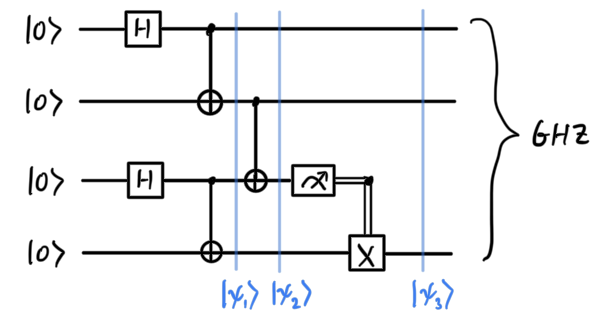
\includegraphics[scale=0.4]{img/propagating_entanglement.png}
        \caption{Circuit diagram for generating the GHZ state from Bell states.} 
        \label{fig:propagating_entanglement}
      \end{figure}
      By generating the GHZ state, we are essentially propagating the entanglement from A to C. 
      \begin{enumerate} 
        \item We start off with the state 
          \begin{equation} 
            \ket{\psi_1} = \ket{\Phi^+} \ket{\Phi^+} = \frac{\ket{0000} + \ket{0011} + \ket{1100} + \ket{1111}}{2}
          \end{equation}
        \item Now we want to make a measurement on only 1 qubit to turn this into a 3 qubit system. The measurement operator that we can use is one that computes whether the 2 qubits that B has match onto the third qubit. This can be done with the parity operator done on B's qubits, as you can see in the following. 
          \begin{align} 
            \ket{00} \mapsto \ket{0\mathbf{0}} \\ 
            \ket{01} \mapsto \ket{1\mathbf{1}} \\ 
            \ket{10} \mapsto \ket{0\mathbf{1}} \\ 
            \ket{11} \mapsto \ket{1\mathbf{0}} 
          \end{align}
          This turns out to be the CNOT with the 2nd qubit being the control and the 3rd being the target. 
          \begin{align} 
            \ket{\psi_2} = \frac{\ket{0000} + \ket{0011} + \ket{1110} + \ket{1101}}{2} 
          \end{align}
        \item Now note that the first and fourth terms have the same third qubit of $0$ and the second/third have the same third qubit of $1$. If we measure the third qubit and it turns out to be $0$, the entangled system will collapse to the first and fourth terms, which is the GHZ state. If it turns out to be $1$, it will collapse to the second and third terms. 
          \begin{align} 
            0 \text{ measured } & \implies \psi_3^\ast = \frac{\ket{000} + \ket{111}}{\sqrt{2}} = \ket{\mathrm{GHZ}} \\
            1 \text{ measured } & \implies \psi_3^\ast = \frac{\ket{001} + \ket{110}}{\sqrt{2}}
          \end{align}
        The second is not the GHZ state but can be turned into one by simply swapping the third qubit between $0$ and $1$. Since this is conditioned on the fact that the measured third (previous) qubit is $1$, we can use a controlled gate with the $X$ since we want them to negated (NOT). Therefore, 
        \begin{equation} 
          \ket{\psi_3} = \frac{\ket{000} + \ket{111}}{\sqrt{2}} = \ket{\mathrm{GHZ}} 
        \end{equation}
      \end{enumerate}
    \end{theorem}

    \begin{question}[To Do] 
      Class 4, how do I create a 4-qubit GHZ state? 
    \end{question}

  \subsection{Quantum Teleportation} 

    We have just proved that we cannot copy qubits, but what is possible is to transfer the state of one qubit to another. This is known as \textbf{quantum teleportation}, or more specifically \textbf{entanglement-assisted teleportation}. More specifically, suppose A has a qubit in quantum state $|\psi \rangle = \alpha |0\rangle + \beta |1 \rangle$ and wants to send this qubit to B (by "sending" it to B, we mean that we want B to be in possession of a qubit in state $|\psi \rangle$ in some way). This is possible under very special circumstances, which we will describe in the theorem below.  

    \begin{theorem}[Quantum Teleportation]
      Given that two parties A wants to send B a qubit $\ket{\psi}$, it is possible to do so under the following assumptions: 
      \begin{enumerate}
        \item An EPR pair (two qubits in some Bell state) has been generated with each qubit given to A and B. This can be done beforehand by A, B, or even a third party C. 
        \item A can communicate to B by sending classical information to B (i.e. finite strings of $0$ and $1$). The finiteness of this condition is most restrictive, since if A could send infinite strings, A can just send the infinite binary representation of $|\psi\rangle$.
      \end{enumerate}
      The entire circuit is represented by the diagram below: 
      \begin{figure}[H]
        \centering 
        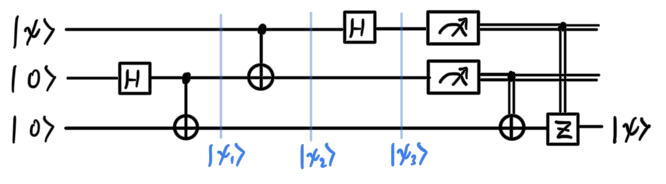
\includegraphics[scale=0.4]{img/quantum_teleportation.png}
        \caption{Quantum teleportation circuit, with A having the first and second qubits and B having the third qubit. } 
        \label{fig:quantum_teleportation}
      \end{figure}
      The following steps are taken: 
      \begin{enumerate} 
        \item Before the experiment, we take the $\ket{00}$ qubit and entangle it, bringing us to $\ket{\psi_1}$. 
          \begin{align} 
            \ket{\psi_1} & = \ket{\psi} \ket{\Phi^+} \\
                         & = \frac{1}{\sqrt{2}} \big( \alpha \ket{0} + \beta \ket{1} \big) \big( \ket{00} + \ket{11} \big) \\
                         & = \frac{1}{\sqrt{2}} \big( \alpha \ket{000} + \alpha \ket{011} + \beta \ket{100} + \beta \ket{111} \big)
          \end{align}
        \item Then, we put take the first and second qubit through a control NOT gate. Since the control is the first qubit, we can just swap the second qubit from $0$ to $1$ or $1$ to $0$ if the first qubit is a $1$ for every component. 
          \begin{align} 
            \ket{\psi_2} & = \frac{1}{\sqrt{2}} \big( \alpha \ket{000} + \alpha \ket{011} + \beta \ket{110} + \beta \ket{101} \big)
          \end{align}
        \item Then, we put the first qubit through a Hadamard gate, which after some computation give us 
          \begin{align*} 
            \ket{\psi_3} & = \frac{1}{2} \bigg( \frac{\alpha}{\sqrt{2}} (\ket{0} + \ket{1}) \ket{00} + \frac{\alpha}{\sqrt{2}} (\ket{0} + \ket{1}) \ket{11}  + \frac{\beta}{\sqrt{2}} (\ket{0} - \ket{1} ) \ket{10} + \frac{\beta}{\sqrt{2}} ( \ket{0} - \ket{1}) \ket{01} \bigg) \\
                         & = \frac{1}{2} \bigg( \alpha \big( \ket{000} + \ket{100} + \ket{011} + \ket{111} + \big) + \beta \big( \ket{010} - \ket{110} + \ket{001} - \ket{101} \big)\bigg) \\
                         & = \frac{1}{2} \bigg( \ket{00} \big( \alpha \ket{0} + \beta \ket{1} \big) + \ket{01} \big( \alpha \ket{1} + \ket{0} \big) + \ket{10} \big( \alpha \ket{0} - \beta \ket{1} \big) + \ket{11} \big( \alpha \ket{1} - \beta \ket{0} \big) \bigg) \\
                         & = \frac{1}{2} \bigg( \ket{00} \big( I \ket{\psi}\big) + \ket{01} \big( X \ket{\psi} \big)  + \ket{10} \big(Z \ket{\psi}\big) + \ket{11} \big( X Z \ket{\psi} \big) \bigg)
          \end{align*}
        \item At this point $\ket{\psi_3}$ stores the state of $\ket{\psi}$, but there needs to be a bit of postprocessing, which can be done with the next gate that takes in the first two classical bits as the control. Depending on what classical bits we measure from the first and second bits, we can undo the operations we did to the third qubit. 
          \begin{enumerate} 
            \item If we measure $00$, then we have $I \ket{\psi}$, and we don't need to do anything. 
            \item If we measure $01$, then we have $X \ket{\psi}$, and we can undo this by applying $X$ again. 
            \item If we measure $10$, then we have $Z \ket{\psi}$, and we can undo this by applying $Z$ again.
            \item If we measure $11$, then we have $X Z \ket{\psi}$, and we can undo this by applying $X$ first and then $Z$. 
          \end{enumerate}
      \end{enumerate}
    \end{theorem}

    Note that A must communicate to B the measurement outcome of the first two bits over a classic communication channel in order to complete the teleportation. Since this classic information is subject to the limits of speed of light, the teleportation of a qubit does not violate the upper limit. This example may also look like it has violated the No-Cloning theorem, since we have copied the qubit $|\psi\rangle$ from A to B. This is not true, since A's $|q_1\rangle$ qubit collapsed onto either a $|0\rangle$ or $|1\rangle$ upon measurement during the process of teleportation (and so we are left with exactly one copy $|\psi\rangle$ in B's possession).

  \subsection{Superdense Coding} 

    In quantum teleportation, we used two classical bits to send a qubit. Superdense coding is simply the reverse: a method to send two bits of information using one qubit.  

    \begin{theorem}[Superdense Coding] 
      Given that A wants to send B two bits of information with just a single qubit, it is possible to do so under the following assumptions: 
      \begin{enumerate} 
        \item A Bell state has been generated with each qubit given to A and B. This can be done beforehand by A, B, or even a third party C.
        \item There exists a channel where A can send a qubit to B.
      \end{enumerate}
      The entire circuit is represented by the diagram below: 
      \begin{figure}[H]
        \centering 
        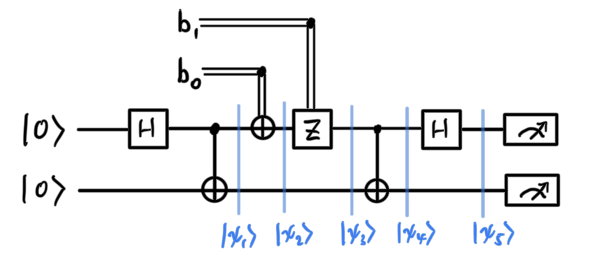
\includegraphics[scale=0.4]{img/superdense_coding.png}
        \caption{Superdense coding circuit, with A having the first qubit with the 2 classical bits and B having the second qubit. Once A manipulates the first qubit, A sends the first qubit to B, who then measures the first and second qubits to get the 2 classical bits. } 
        \label{fig:superdense_coding}
      \end{figure}
      The following steps are taken. 
      \begin{enumerate} 
        \item Before the experiment, we take the $\ket{00}$ qubit and entangle it, bringing us to $\ket{\psi_1}$. 
          \begin{equation} 
            \ket{\psi_1} = \frac{1}{\sqrt{2}} \big( \ket{00} + \ket{11} \big)
          \end{equation}
        \item Then we do a control NOT with a classical control bit $b_0$. 
          \begin{equation} 
            \ket{\psi_2} = \frac{1}{\sqrt{2}} \big( \ket{0 b_0} + \ket{1, 1 \oplus b_0} \big)
          \end{equation}
        \item Then we do a control Z with a classical control bit $b_1$
          \begin{equation} 
            \ket{\psi_3} = \frac{1}{\sqrt{2}} \big( \ket{0 b_0} + (-1)^{b_1} \ket{1, 1 \oplus b_0} \big)
          \end{equation}
        \item Then we do a quantum control NOT with the control qubit as the first qubit that A has, which unentangles the system! 
          \begin{equation} 
            \ket{\psi_4} = \frac{1}{\sqrt{2}} \big( \ket{0 b_0} + (-1)^b \ket{1 b_1} \big) = \bigg( \frac{\ket{0} + (-1)^{b_1} \ket{1}}{\sqrt{2}} \bigg) \ket{b_0} 
          \end{equation}
        \item Then we do a Hadamard on the first qubit unentangling it. 
          \begin{equation} 
            \ket{\psi_5} = (H \otimes I) \ket{\psi_4} = \ket{b_1 b_0} 
          \end{equation}
        \item Now the first qubit, in possession by A, is sent to $B$, which is now in state $\ket{b_1 b_0}$. 
      \end{enumerate}
    \end{theorem}

    \begin{example}[Superdense Coding with Two Classical 0 Bits]
      Since it is a bit more tedious to prove, we will show for the $(b_0, b_1) = (0, 0)$ case and show for the $(b_0, b_1) = (0, 1)$ case in a future example.
      \begin{enumerate} 
        \item Before the experiment, we take the $\ket{00}$ qubit and entangle it, bringing us to $\ket{\psi_1}$. 
          \begin{equation} 
            \ket{\psi_1} = \frac{1}{\sqrt{2}} \big( \ket{00} + \ket{11} \big)
          \end{equation}
        \item Then we do a control NOT with a classical control bit $b_0 = 0$. Nothing changes. 
          \begin{equation} 
            \ket{\psi_2} = \frac{1}{\sqrt{2}} \big( \ket{00} + \ket{11} \big)
          \end{equation}
        \item Then we do a control Z with a classical control bit $b_1 = 0$. Nothing changes. 
          \begin{equation} 
            \ket{\psi_3} = \frac{1}{\sqrt{2}} \big( \ket{00} + \ket{11} \big)
          \end{equation}
        \item Then we do a quantum control NOT with the control qubit as the first qubit that A has. 
          \begin{equation} 
            \ket{\psi_4} = \frac{1}{\sqrt{2}} \big( \ket{00} + \ket{10} \big) = \frac{1}{\sqrt{2}} \big( \ket{0} + \ket{1} \big) \ket{0}
          \end{equation}
        \item Then we do a Hadamard on the first qubit unentangling it. 
          \begin{equation} 
            \ket{\psi_5} = (H \otimes I) \ket{\psi_4} = \ket{00}
          \end{equation}
        \item Now the first qubit, in possession by A, is sent to $B$. 
        \item The final qubit is of state $\ket{00}$, which is guaranteed to have measurement $(0, 0) = (b_0, b_1)$ as A had, and so B measures the first and second qubits to get the 2 classical bits. 
      \end{enumerate}
    \end{example}

    \begin{example}[Superdense Coding with Two Classical 1 Bits]
      As promised, we outline the steps for when A has $(b_0, b_1) = (1, 1)$.
      \begin{enumerate} 
        \item Before the experiment, we take the $\ket{00}$ qubit and entangle it, bringing us to $\ket{\psi_1}$. 
          \begin{equation} 
            \ket{\psi_1} = \frac{1}{\sqrt{2}} \big( \ket{00} + \ket{11} \big)
          \end{equation}
        \item Then we do a control NOT with a classical control bit $b_0 = 1$. The first qubit is flipped. 
          \begin{equation} 
            \ket{\psi_2} = \frac{1}{\sqrt{2}} \big( \ket{10} + \ket{01} \big)
          \end{equation}
        \item Then we do a control Z with a classical control bit $b_1 = 1$. The $\ket{1}$ component of the first qubit changes sign from $+$ to $-$. 
          \begin{equation} 
            \ket{\psi_3} = \frac{1}{\sqrt{2}} \big( - \ket{10} + \ket{01} \big)
          \end{equation}
        \item Then we do a quantum control NOT with the control qubit as the first qubit that A has. 
          \begin{equation} 
            \ket{\psi_4} = \frac{1}{\sqrt{2}} \big( -\ket{11} + \ket{01} \big) = \frac{1}{\sqrt{2}} \big( \ket{0} - \ket{1} \big) \ket{1}
          \end{equation}
        \item Then we do a Hadamard on the first qubit unentangling it. 
          \begin{equation} 
            \ket{\psi_5} = (H \otimes I) \ket{\psi_4} = \ket{11}
          \end{equation}
        \item Now the first qubit, in possession by A, is sent to $B$. 
        \item The final qubit is of state $\ket{11}$, which is guaranteed to have measurement $(1, 1) = (b_0, b_1)$ as A had, and so B measures the first and second qubits to get the 2 classical bits. 
      \end{enumerate}
    \end{example}

  \subsection{Quantum Parallelism}

    There are two limitations of quantum computing. The first one is that the gates must be $n \times n$ and therefore the number of qubits coming in must equal the number of qubits coming out. This is not too bad, since we can add, remove, or measure in some clever way. The bigger limitation is that quantum gates must be reversible, and therefore they cannot simulate functions that are not invertible. For example, say the function $f: \{0, 1\} \longrightarrow \{0, 1\}$ is defined by $f(0) = f(1) = 1$. This is not invertible, and so we cannot simulate this function with a quantum gate. What we can do is simply extend the codomain so that no outputs overlap with each other. That is, we can simply say $f(0) = 01$ and $f(1) = 11$, setting the first bit to be a dummy variable and the second bit to be the actual output. But now we've broken the first rule since the number of qubits coming out is not the same as the number of qubits coming in. Therefore, we simply increase the dimensionality of the domain as well. Therefore, we can say that $f(00) = 01$ and $f(10) = 11$, where the second bit of the input is now a dummy variable. Problem solved. It is not too hard to see the general case. 

    \begin{lemma}[Reversible Computing of a Classical Function]
      Given a classical function $f: \{0, 1\}^n \longrightarrow \{0, 1\}^m$, we can simulate this function with a reversible quantum gate $U_f: \{0, 1\}^{n+m} \longrightarrow \{0, 1\}^{n+m}$, where $n$ is the number of input bits and $m$ is the number of output bits.
    \end{lemma}
    \begin{proof} 
      We don't give a formal proof here, but consider the worst case scenario where $f = 0^m$ always. Since all the outputs are the same, the inputs must be distinct, so we need at least $n$ dimensions to store the keys of the inputs. The actual output size is $m$, so we also need an extra $m$ dimensions to store the outputs, leading to $n + m$. 
    \end{proof}

    Therefore, we have the set of inputs $x \in \{0, 1\}^n$ and the set of outputs $\{f(x)\}$. It is conventional to do the following: 
    \begin{enumerate} 
      \item Since the inputs must be of dimension $n+m$, we just write the first $n$ bits as the actual inputs and the last $m$ bits as dummy variables, call it $y$, which can be set to all $0$ or all $1$ for simplicity.  
      \item Since the outputs is of dimension $n+m$, the first $n$ bits will be set to the dummy variables, which are set to the input values, and the last $m$ bits will be the actual outputs. 
    \end{enumerate}

    For now, let's focus on when $m = 1$. 

    \begin{example}[Toffoli Gate as extension of NAND Gate]
      The Toffoli gate can simulate the NAND gate as its extension. To see how, the input is of form $\mathbf{x} y = \mathbf{x_1 x_2 y} = x_1 x_2 1$, where we have set $y$ to all $1$. Then looking at the output of the Toffoli gate, we can see that in its respective outputs, the first two bits are simply the inputs and the third bit is the NAND of the first two bits, the actual output. 

      \begin{center}
        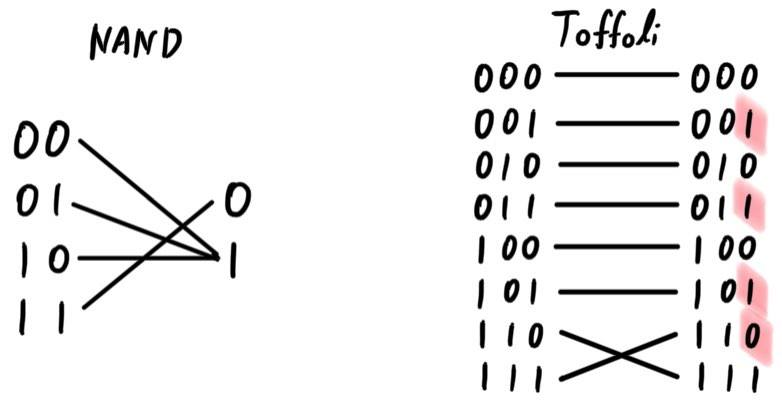
\includegraphics[scale=0.3]{img/Toffoli_NAND_extension.jpg}
      \end{center}
      More formally, we can write 
      \begin{equation} 
        \text{NAND}(xy) = \delta_3 \circ \text{Toffoli}(xy1)
      \end{equation}
      where $\delta_3: xyz \mapsto z$. Since the Toffoli gate allows us to simulate the universal NAND gate, it becomes possible to simulate all other elements in a classical circuit and thus an arbitrary classical circuit can be simulated by an equivalent reversible circuit.
    \end{example}

    \begin{definition}[Reversible Extension of Functions]
      In general, given a function $f: \{0, 1\}^n \rightarrow \{0, 1\}$, we can set the dummy variable $y = 0$ always and construct a reversible extension $U_f$ defined 
      \begin{equation} 
        U_f: \{0, 1\}^{n+1} \longrightarrow \{0, 1\}^{n+1}, \; U_f: \, |x \rangle |y\rangle \mapsto |x\rangle |y \oplus f(x) \rangle.
      \end{equation} 
      and since $y = 0$, $y \oplus f(x) = f(x)$.
    \end{definition}

    Constructing this reversible extension of classical functions gives us the foundation to work with \textbf{quantum parallelism}, which is a fundamental feature of many quantum algorithms that, heuristically, allows quantum computers to evaluate a function $f(x)$ for many different values of $x$ simultaneously. More specifically, by inputting a superposition of all possible inputs into a reversible extension of a function, we can obtain a superposition of all possible outputs. 

    \begin{example}[Function of 1-Bit Input]
      Suppose $f: \{0, 1\} \longrightarrow \{0, 1\}$ is a function. To evaluate $f$ on all possible bits, we need to call $f$ 2 times: $f(0), f(1)$. We can create a reversible extension of this function $f$ by extending the domain and codomain to $\{0, 1\}^2$ to construct
      \begin{equation} 
        U_f: \{0, 1\}^2 \longrightarrow \{0, 1\}^2, \; U_f: \, |x \rangle |y\rangle \mapsto |x\rangle |y \oplus f(x) \rangle
      \end{equation}
      With the construction of $U_f$, all we need to do is pay attention to all the outputs where the input has $y=0$, since $U_f (|x \rangle |0\rangle) = |x \rangle \, |f(x) \rangle$.
      \begin{center}
        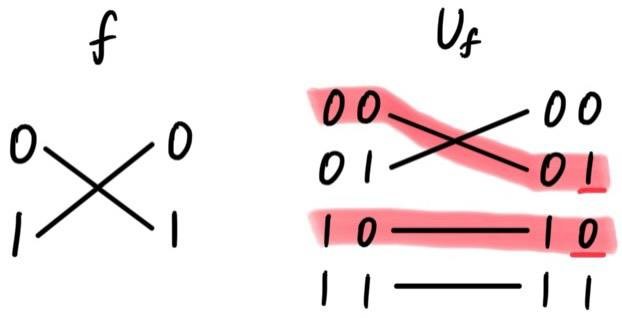
\includegraphics[scale=0.3]{img/f_to_U_one_qubit_reversible.jpg}
      \end{center}
      By setting $\ket{y} = \ket{0}$ and with it, (the important part) inputting in a superposition of all possible inputs (which we can just get by doing a Hadamard) $\ket{x} = H \ket{0} = \frac{\ket{0} + \ket{1}}{\sqrt{2}}$, we can obtain a superposition of all possible outputs.
      \begin{align*}
        U (|x\rangle \otimes |y\rangle) & = U \bigg(\frac{\ket{0} + \ket{1}}{\sqrt{2}} \otimes \ket{0} \bigg) \\ 
                                        & = U \bigg( \frac{\ket{00} + \ket{10}}{\sqrt{2}} \bigg) \\ 
                                        & = \frac{U \ket{00} + U \ket{10}}{\sqrt{2}} \\ 
                                        & = \frac{\ket{0} \ket{f(0)} + \ket{1} \ket{f(1)}}{\sqrt{2}}
      \end{align*}

      This output state is very interesting because the different terms contain information about both $f(0)$ and $f(1)$. It is almost as if we evaluated $f(x)$ for two values of $x$ simultaneously. Note that unlike classical parallelism, where multiple circuits each built to compute $f(x)$ are executed simultaneously, here a single $f(x)$ circuit is employed to evaluate the function for multiple values of $x$ simultaneously.
    \end{example}

    \begin{example}[Function of 2-Bit Input]
      Suppose $f: \{0, 1\}^2 \longrightarrow \{0, 1\}$ is a function. To evaluate $f$ on all four permutations of two bits, we need to call $f$ 4 times: $f(00), f(01), f(10), f(11)$. We can create a reversible extension of this function $f$ by extending the domain and codomain to $\{0, 1\}^3$ to construct
      \begin{equation} 
        U_f: \{0, 1\}^3 \longrightarrow \{0, 1\}^3, \;\; U_f: \, |x_1 x_2 \rangle\,|y\rangle \mapsto |x_1 x_2 \rangle\, |y \oplus f(x_1 x_2) \rangle
      \end{equation}
      With the construction of $U_f$ shown below, all we need to do is pay attention to all the outputs where the input has $y=0$, since $U_f (|x_1 x_2 \rangle |0\rangle) = |x_1 x_2 \rangle \, |f(x) \rangle$.
      \begin{center}
        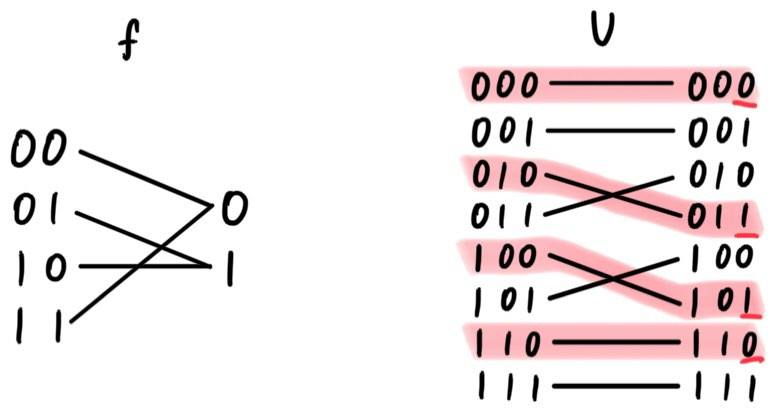
\includegraphics[scale=0.3]{img/f_to_U_reversible.jpg}
      \end{center}
      Again, we set $\ket{y} = 0$ and now we want a superposition of all possible two-qubit inputs. What better way to do this than to apply the Hadamard transform $H^{\otimes 2}$ to the first two qubits? 
      \begin{align} 
        U (\ket{x} \otimes \ket{y}) & = U \big( H^{\otimes 2} \ket{00} \otimes \ket{0} \big) \\
                                    & = \ldots \\
                                    & = \frac{\ket{00} \ket{f(00)} + \ket{01} \ket{f(01)} + \ket{10} \ket{f(10)} + \ket{11} f(\ket{11})}{2}
      \end{align}
      Again, this output state is interesting because it contains information about all its input values. It is almost as if we evaluated $f(x)$ simultaneously.
    \end{example}
    
    If you can simulate a NAND gate with a Toffoli, and NAND is the universal gate for classical computing, then can't we construct cloning gates (like XOR)? The answer is no, since we can only do it for classical bits, not quantum bits. Let's generalize this procedure for $N$-bit inputs. 

    \begin{theorem}[Quantum Parallelism of N-bit Input]
      Given some function $f: \{0, 1\}^n \longrightarrow \{0, 1\}$, we can take the state $|0\rangle^{\otimes (n+1)}$ and apply the Hadamard transformation $H^{\otimes n}$ on the first $n$ qubits to prepare the $(n+1)$-qubit state 
      \begin{equation} 
        |x_1 \ldots x_n \rangle \otimes |y\rangle = \left( \frac{|0\rangle + |1\rangle}{\sqrt{2}}\right)^{\otimes n} \otimes |0\rangle
      \end{equation}
      Then, we put it through the (reversible) quantum circuit $U_f: \{0, 1\}^{n+1} \longrightarrow \{0, 1\}^{n+1}$ constructed as an extension of the classical $f$ defined 
      \begin{equation} 
        U_f \, |x_1 x_2 \ldots x_n \rangle \, |y\rangle \mapsto |x_1 x_2 \ldots x_n \rangle \, |y \oplus f(x_1 \ldots x_n)\rangle
      \end{equation}
      which gives 
      \begin{equation} 
        U_f \big( H^{\otimes n} \ket{0}^{\otimes n} \otimes \ket{0} \big) = U_f \Bigg( \bigg( \frac{|0\rangle + |1\rangle}{\sqrt{2}} \bigg)^{\otimes n} \otimes |0\rangle \Bigg) = \frac{1}{\sqrt{2^n}} \sum_{x \in \{0, 1\}^n} |x\rangle \, |f(x)\rangle
      \end{equation}
      This output state contains information about all of the possible values $f(x)$. But the question still remains what to do with this output 
      \begin{equation} 
        \frac{1}{\sqrt{2^n}} \sum_{x \in \{0, 1\}^n} |x\rangle \, |f(x)\rangle
      \end{equation}
    \end{theorem}

    While this one state contains all the information defining the function $f$ on the one hand, it is still in superposition that will collapse onto \textit{one} measurement outcome $|x \rangle \otimes |f(x) \rangle$. Therefore, quantum computation requires something more than just quantum parallelism to be useful; it requires the ability to \textit{extract} information about more than one value of $f(x)$ from superposition states. This is where the Deutsch algorithm comes in. 

\section{Quantum Fourier Transform} 

  \subsection{Deutsch Algorithm}

    With quantum parallelism, we've evaluated a superposition of the inputs to get a superposition of the outputs. Unfortunately, we can't just extract all information from this output, but there are some \textit{global properties} of the function that we can deduce, with \textit{interference}. What do we mean by global properties? Let's look at an example below. 

    \begin{example}[1 Bit Function]
      Given a function $f: \{0, 1\} \longrightarrow \{0, 1\}$, we can determine the following equivalent properties: 
      \begin{enumerate} 
        \item whether the $f$ is constant or balanced, i.e. whether it is constantly $0$ or $1$.
        \item the value of $f(0) \oplus f(1)$
        \item whether $f$ is surjective or not. 
      \end{enumerate}
      It is easy to see how knowing one property allows you to know other properties. 
    \end{example}

    To get these global properties, it usually requires us to run a classical circuit over all inputs of $f$, which may not be computationally feasible. Finding the surjectivity of a $1$-bit input function above will require $2$ forward passes, but we claim that we can do it on a quantum circuit with just one forward pass. To do this, it requires a bit of clever thinking, where the dummy variable $\ket{y}$ is now also set to a Bell state. 

    \begin{theorem}[Deutsch Algorithm for 1-Bit Input Function]  
      Let Alice and Bob be isolated except for a channel where they may send one qubit to each other. Given that Bob has a one-bit input function $f: \{0, 1\} \longrightarrow \{0, 1\}$, it is possible for Alice to determine the value of $f(0) \oplus f(1)$ with just one forward pass of $f(x)$ on a quantum circuit without knowing Bob's function. The circuit is shown first for clarity: 
      \begin{figure}[H]
        \centering 
          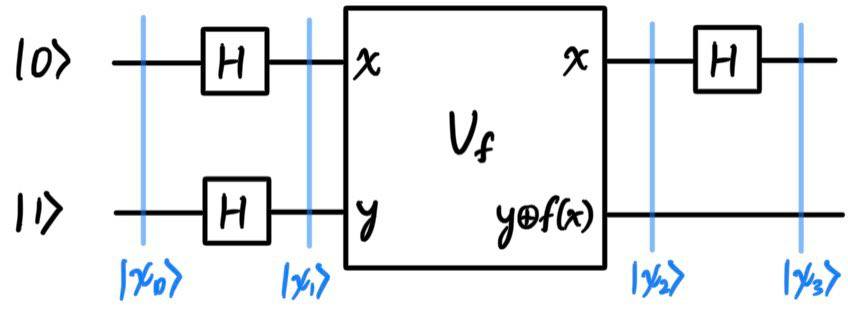
\includegraphics[scale=0.3]{img/Deutsch_Algo.jpg}
        \caption{Deutsch Algorithm for 1-bit input function.} 
        \label{fig:Deutsch_Algo}
      \end{figure}
      Like we have always done, we can take the reversible extension $U_f: |x\rangle |y\rangle \mapsto |x \rangle |y \oplus f(x)\rangle$. The following steps are taken. 
      \begin{enumerate} 
        \item Alice prepares a bell state by taking a Hadamard on each input qubit. 
          \begin{equation} 
            \ket{\psi_1} = H^{\otimes 2} \ket{01} = \ket{\Phi^+} \otimes \ket{\Phi^-} 
          \end{equation}
        \item Alice sends $\ket{\psi_1}$ to Bob, and Bob now passes it through $U_f$, but before this, observe that for any arbitrary input $x$, we have  
          \begin{align} 
            U_f \bigg( \ket{x} \otimes \frac{\ket{0} - \ket{1}}{\sqrt{2}} \bigg) 
            & = \frac{U_f (\ket{x} \ket{0}) - U_f (\ket{x} \ket{1})}{\sqrt{2}} \\
            & =  \frac{\ket{x} \otimes \ket{0 \oplus f(x)} - \ket{x} \otimes \ket{1 \oplus f(x)}}{\sqrt{2}} \\ 
            & = \frac{\ket{x} \otimes \big( \ket{0 \oplus f(x)} - \ket{1 \oplus f(x)} \big)}{\sqrt{2}} \\ 
            & = \begin{cases} 
              \frac{\ket{x} \otimes ( \ket{0} - \ket{1})}{\sqrt{2}} & \text{if } f(0) = f(1), \\
              \frac{-\ket{x} \otimes ( \ket{0} - \ket{1})}{\sqrt{2}} & \text{if } f(0) \neq f(1) 
            \end{cases} \\
            & = \frac{(-1)^{f(x)} \ket{x} \big( \ket{0} - \ket{1} \big)}{\sqrt{2}}
          \end{align}
          Therefore, for $\ket{x} = \ket{\Phi^+}$, we have 
          \begin{align} 
            \ket{\psi_2} = U_f \ket{\psi_1} & = U_f \bigg( \frac{\ket{0} + \ket{1}}{\sqrt{2}} \otimes \frac{\ket{0} - \ket{1}}{\sqrt{2}} \bigg) \\
                             & = \frac{1}{\sqrt{2}} U_f \bigg( \ket{0} \otimes \frac{\ket{0} - \ket{1}}{\sqrt{2}} \bigg) + \frac{1}{\sqrt{2}} U_f \bigg( \ket{1} \otimes \frac{\ket{0} - \ket{1}}{\sqrt{2}} \bigg) \\ 
                             & = \frac{(-1)^{f(0)} \ket{0} ( \ket{0} - \ket{1})}{\sqrt{2} \cdot \sqrt{2}} + \frac{(-1)^{f(1)} \ket{1} ( \ket{0} - \ket{1})}{\sqrt{2} \cdot \sqrt{2}} \\  
                             & = \begin{cases} 
                               \pm \bigg( \frac{\ket{0} + \ket{1}}{\sqrt{2}} \bigg) \bigg( \frac{\ket{0} - \ket{1}}{\sqrt{2}} \bigg) & \text{if } f(0) = f(1), \\
                               \pm \bigg( \frac{\ket{0} - \ket{1}}{\sqrt{2}} \bigg) \bigg( \frac{\ket{0} - \ket{1}}{\sqrt{2}} \bigg) & \text{if } f(0) \neq f(1)
                             \end{cases}
          \end{align}
        \item Bob sends $\ket{\psi_2}$ back to Alice, who now applies the Hadamard gate on the first qubit now gives us 
          \begin{align} 
            \ket{\psi_3} & = (H \otimes I) \ket{\psi_2} = \begin{cases} 
              \pm \ket{0} \bigg( \frac{\ket{0} - \ket{1}}{\sqrt{2}} \bigg) & \text{if } f(0) = f(1), \\ 
              \pm \ket{1} \bigg( \frac{\ket{0} - \ket{1}}{\sqrt{2}} \bigg) & \text{if } f(0) \neq f(1)
            \end{cases} \\
                         & = \pm \ket{f(0) + f(1)} \bigg( \frac{\ket{0} - \ket{1}}{\sqrt{2}} \bigg) 
          \end{align}
        \item Therefore, by measuring the first qubit, we can determine $f(0) \oplus f(1)$, i.e., whether $f(0) = f(1)$ or $f(0) \neq f(1)$. 
      \end{enumerate}
    \end{theorem}

  \subsection{The Deutsch-Jozsa Algorithm}

    This type of problem where we must efficiently guess this property of a function is called Deutch's problem. 

    \begin{definition}[Deutch's Problem]
      Alice selects a number $x$ from $0$ to $2^n - 1$, which can be represented as an element in $\{0, 1\}^n$ (isomorphic?) and mails it in a letter to Bob. Bob calculates some function $f: \{0, 1\}^n \longrightarrow \{0, 1\}$ and replies with the result, which is either $0$ or $1$. Bob promises to use a function $f$ which is one of two kinds: 
      \begin{enumerate}
        \item $f(x)$ is constant for all values of $x$, or
        \item $f(x)$ is balanced, meaning that it outputs $1$ for exactly half of the possible $x$ and $0$ for the other half (note that this does \textit{not} mean that $f$ outputs $0$ and $1$ probabilistically; $f$ is completely deterministic). 
      \end{enumerate}
    \end{definition}

    However, this problem is not known to have any applications, and probabilistic computation can be similarly used to solve this problem with a high (but not certain) degree of accuracy. 

    Again, in the classical case, Alice may send Bob one value of $x$ in each letter. At worst, she will need to query Bob at least $2^{n-1} + 1$ times (half of possible inputs, plus one) and therefore the best deterministic classical algorithm she can use therefore requires $2^{n-1} + 1$ queries (i.e. a computational complexity of $O(2^n)$). However, we claim that if Bob and Alice were able to exchange qubits instead of classical bits, and Bob agreed to calculate $f(x)$ using a unitary transformation $U_f$, then Alice can achieve her goal of just \textit{one} correspondence with Bob. Before we start, let's introduce a lemma. 

    \begin{lemma}
      Given a state $\ket{x}$, the Hadamard gate $H$ acts on it as 
      \begin{equation} 
        H \ket{x} = \sum_{z \in \{0, 1\}} \frac{(-1)^{x \cdot z} \ket{z}}{\sqrt{2}} 
      \end{equation}
      and for general state $\ket{\mathbf{x}} = \ket{x_1 x_2 \ldots x_n}$, we have 
      \begin{equation} 
        H^{\otimes n} \ket{\mathbf{x}} = \sum_{\mathbf{z} \in \{0, 1\}^n} \frac{(-1)^{\mathbf{x} \cdot \mathbf{z}} \ket{\mathbf{z}}}{\sqrt{2^n}}
      \end{equation}
      where $\mathbf{x} \cdot \mathbf{z}$ is the bitwise dot product of $\mathbf{x}, \mathbf{z} \in \{0, 1\}^n$ modulo $2$. 
    \end{lemma}
    \begin{proof} 
      We can see that for $|x\rangle = |0\rangle$ or $|1\rangle$, 
      \begin{equation} 
        H|x\rangle = \sum_{z \in \{0, 1\}} \frac{(-1)^{xz} |z\rangle}{\sqrt{2}} = \frac{|0\rangle + (-1)^x |1\rangle}{\sqrt{2}}
      \end{equation}
      Now given $\ket{x} = \ket{x_1 x_2 \ldots x_n}$, we can take the tensor products of these terms. 

      \begin{align*} 
        H^{\otimes n} \ket{\mathbf{x}} 
        & = H \ket{x_1} \otimes H \ket{x_2} \otimes \ldots \otimes H \ket{x_n} \\
        & = \bigg( \sum_{z_1 \in \{0, 1\}} \frac{1}{\sqrt{2}} (-1)^{x_1 z_1} \ket{z_1} \bigg) \otimes \ldots \otimes \bigg( \sum_{z_n \in \{0, 1\}} \frac{(-1)^{x_n z_n} \ket{z_n}}{\sqrt{2}} \bigg) \\
        & = \sum_{\mathbf{z} \in \{0, 1\}^n} \frac{(-1)^{x_1 z_1} \ket{z_1} \otimes \ldots \otimes (-1)^{x_n z_n} \ket{z_n}}{\sqrt{2^n}} \\
        & = \sum_{\mathbf{z} \in \{0, 1\}^n} \frac{(-1)^{x_1 z_1 + \ldots + x_n z_n} \, |z_1 \ldots z_n \rangle}{\sqrt{2^n}} \\
        & = \sum_{\mathbf{z} \in \{0, 1\}^n} \frac{(-1)^{\mathbf{x} \cdot \mathbf{z}} \, \ket{\mathbf{z}}}{\sqrt{2^n}}
      \end{align*}
    \end{proof}

    \begin{theorem}[Deutsch Jozsa Algorithm]
      Let Alice and Bob be isolated except for a channel where they may send qubits to each other. Alice can solve Deutch's problem with a single pass on a quantum circuit. The circuit is shown first for clarity:
      \begin{figure}[H]
        \centering 
        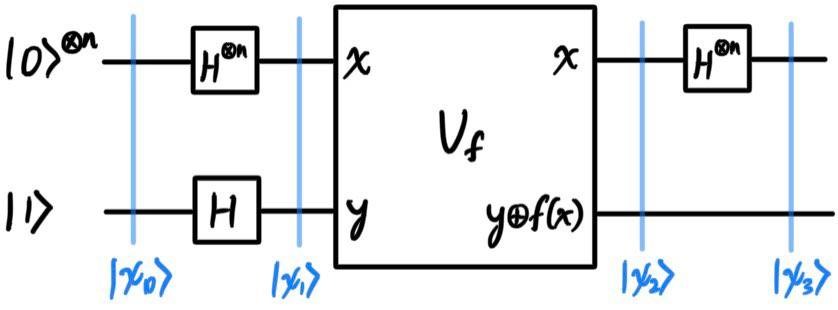
\includegraphics[scale=0.3]{img/Deutsch_Jozsa_Algo.jpg}
        \caption{Deutsch-Jozsa Algorithm.} 
        \label{fig:Deutsch_Jozsa_Algo}
      \end{figure}
      Bob constructs the reversible extension $U_f: |x\rangle |y\rangle \mapsto |x \rangle |y \oplus f(x)\rangle$. The following steps are taken.
      \begin{enumerate} 
        \item Alice prepares a state $\ket{\psi_1} = H^{\otimes n} \ket{0}^{\otimes n} \otimes \ket{1}$ and sends it to Bob. 
          \begin{equation} 
            \ket{\psi_1} = H^{\otimes (n+1)} (\ket{0}^{\otimes n} \otimes \ket{1}) = \frac{1}{\sqrt{2^n}} \sum_{x \in \{0, 1\}^n} \ket{x} \bigg[ \frac{\ket{0} - \ket{1}}{\sqrt{2}} \bigg] 
          \end{equation}
        \item Bob applies $U_f$ to $\ket{\psi_1}$ to get 
          \begin{equation} 
            \ket{\psi_2} = U_f \ket{\psi_1} = \sum_{x \in \{0, 1\}^n} \frac{(-1)^f(x) \ket{x}}{\sqrt{2^n}} \bigg[ \frac{\ket{0} - \ket{1}}{\sqrt{2}} \bigg] 
          \end{equation}
        \item Bob sends $\ket{\psi_2}$ back to Alice, who evaluates the Hadamard on the first $n$ qubits. We can use the previous lemma to get 
          \begin{equation} 
            \ket{\psi_3} = H^{\otimes n} \ket{\psi_2} = \sum_\mathbf{z} \sum_{\mathbf{x}} \frac{(-1)^{\mathbf{x} \cdot \mathbf{z} + f(\mathbf{x})} \ket{\mathbf{z}}}{2^n} \bigg[ \frac{\ket{0} - \ket{1}}{\sqrt{2}} \bigg]
          \end{equation}
        \item Alice now measures the query register (i.e., the first $n$ qubits). The complete expansion is too long to write out, but we can focus on the amplitude for the state $\ket{\mathbf{z}} = |0\rangle^{\otimes n}$. 
          \begin{equation} 
            \sum_{z \in \{0, 1\}^n} \sum_{x \in \{0, 1\}^n} \frac{(-1)^{x \cdot z + f(x)}}{2^n} |z\rangle = \left( \sum_{x \in \{0, 1\}^n} \frac{(-1)^{f(x)}}{2^n}\right) |0\ldots 0 \rangle \otimes \frac{|0\rangle - |1\rangle}{\sqrt{2}} + \ldots
          \end{equation}
          Note that the amplitude for the state $|0\rangle^{\otimes n}$ (i.e., when $|z\rangle = |0 \ldots 0\rangle$) is 
          \begin{equation} 
            \sum_{x \in \{0, 1\}^n} \frac{(-1)^{f(x)}}{2^n}
          \end{equation}
          There are two scenarios: 
          \begin{enumerate}
            \item If $f(x)$ is constant for all values of $x$, then this amplitude would be 

            \begin{align*} 
              \sum_{x \in \{0, 1\}^n} \frac{(-1)^{f(x)}}{\sqrt{2^n}} & = \sum_{x \in \{0, 1\}^n} \frac{1}{2^n} = 1 \text{ if } f(x) = 0, \\
              \sum_{x \in \{0, 1\}^n} \frac{(-1)^{f(x)}}{\sqrt{2^n}} & = \sum_{x \in \{0, 1\}^n} \frac{-1}{2^n} = -1 \text{ if } f(x) = 1.
            \end{align*}

            Since $|\psi_3 \rangle$ must be a unit vector, this implies that all the other amplitudes are $0$ and therefore $|\psi_3 \rangle = |0\rangle^{\otimes n}$. 

            \item If $f(x)$ is balanced, then the number of negative terms and positive terms will cancel each other out, and so 

              \[\sum_{x \in \{0, 1\}^n} \frac{(-1)^{f(x)}}{2^n} = 2^{n-1} \cdot 1 + 2^{n-1} \cdot (-1) = 0,\]

            meaning that the amplitude of $|0\rangle^{\otimes n}$ is $0$. 
          \end{enumerate}
          Therefore, by measuring the query register, if everything pops up to $\mathbf{1}$, then it is constant and if everything collapses to $\mathbf{0}$, then it is balanced. 
      \end{enumerate}
    \end{theorem}
    \begin{proof} 
      We've left out a lot of computation here for simplicity. Here we show the full derivations. 
      \begin{enumerate} 
        \item Trivial. 
        \item Again, to calculate $|\psi_2 \rangle$, we use the fact (which does not matter how many bits $x$ is)

          \[U_f |x\rangle \otimes \frac{|0\rangle - |1\rangle}{\sqrt{2}} = (-1)^{f(x)} \,|x\rangle \, \frac{|1\rangle - |0\rangle}{\sqrt{2}},\]

        and sum it over all possible permutations of $x \in \{0, 1\}^n$ to get 

        \begin{align*} 
          U_f |\psi_1 \rangle & = U_f \left( \sum_x \frac{1}{\sqrt{2}} |x\rangle \right) \otimes \frac{|0\rangle - |1\rangle}{\sqrt{2}} \\
          & = U_f \sum_x \left( \frac{1}{\sqrt{2}} |x\rangle \otimes \frac{|0\rangle - |1\rangle}{\sqrt{2}}\right) \\
          & = \sum_x \frac{1}{\sqrt{2}} U_f \left( |x\rangle \otimes \frac{|0\rangle - |1\rangle}{\sqrt{2}} \right) \\
          & = \sum_x (-1)^{f(x)} \frac{|x\rangle}{\sqrt{2^n}} \otimes \frac{|0\rangle - |1\rangle}{\sqrt{2}}
        \end{align*}

        \item $|\psi_3 \rangle$ is calculated with the following steps. 

        \begin{align*} 
          |\psi_3 \rangle & = (H^{\otimes n} \otimes I) |\psi_2 \rangle = H^{\otimes n} \left( \sum_{x \in \{0, 1\}^n} (-1)^{f(x)} \frac{|x\rangle}{\sqrt{2^n}} \right) \otimes I \left( \frac{|0\rangle - |1\rangle}{\sqrt{2}} \right)\\
          & = \left( \sum_{x \in \{0, 1\}^n} \frac{(-1)^{f(x)}}{\sqrt{2^n}} H^{\otimes n} |x\rangle \right) \otimes \frac{|0\rangle - |1\rangle}{\sqrt{2}} \\
          & = \sum_{x \in \{0, 1\}^n} \frac{(-1)^{f(x)}}{\sqrt{2^n}} \left( \frac{1}{\sqrt{2^n}} \sum_{z \in \{0, 1\}^n} (-1)^{x \cdot z} |z \rangle \right) \otimes \frac{|0\rangle - |1\rangle}{\sqrt{2}} \\
          & = \sum_{x \in \{0, 1\}^n} \sum_{z \in \{0, 1\}^n} \frac{1}{2^n} (-1)^{x \cdot z + f(x)} |z\rangle \otimes \frac{|0\rangle - |1\rangle}{\sqrt{2}} \\
          & = \sum_{z \in \{0, 1\}^n} \sum_{x \in \{0, 1\}^n} \frac{1}{2^n} (-1)^{x \cdot z + f(x)} |z\rangle \otimes \frac{|0\rangle - |1\rangle}{\sqrt{2}}
        \end{align*}
      \end{enumerate}
    \end{proof}

    Remember that quantum computation is superior to classical computation if \textit{both} of the following requirements are met: 
    \begin{enumerate}
      \item We can utilize the non-binary superpositions of qubits to calculate more efficiently using quantum parallelism. 
      \item We have some method to \textit{extract} information from the output qubit(s) using measurements. The answers are all there in the qubit state, but they are hidden: measuring it would cause it to collapse onto a string of $|0\rangle$s and $|1\rangle$s, and so a creative method of gaining information is needed. 
    \end{enumerate}

    \begin{theorem}[Quantum Fourier Transform]
      The quantum Fourier transform is a unitary transformation that maps a state $\ket{x}$ to a state $\ket{\tilde{x}}$ according to the rule 
      \begin{align}
      QFT|\mathbf{x}\rangle &= 
      \frac{1}{\sqrt{2^n}} \sum_{k = 0}^{2^n-1} e^{\frac{2 \pi i \mathbf{x} \mathbf{k} }{2^n}} |\mathbf{k}\rangle \\ & = \frac{|0 \rangle + e^{2\pi i (0.x_n)}|1\rangle}{\sqrt{2}} \otimes \frac{|0\rangle + e^{2 \pi i (0.x_{n-1}x_n)}|1\rangle}{\sqrt{2}} \otimes \cdots \otimes \frac{|0\rangle + e^{2 \pi i (0.x_1 x_2\cdots x_n)}|1\rangle}{\sqrt{2}} \ \ \ .
      \end{align}
    \end{theorem}
    \begin{proof} 
      \begin{align} 
        \frac{1}{\sqrt{2^n}} \sum_{k = 0}^{2^n-1} e^{\frac{2 \pi i \mathbf{x} \mathbf{k} }{2^n}} |\mathbf{k}\rangle 
        & = \frac{1}{\sqrt{2^n}} \sum_{k_1 \in \{0, 1\}} \ldots \sum_{k_n \in \{0, 1\}} \exp \bigg( 2 \pi i \mathbf{x} \Big[ \sum_{l=1}^n k_l 2^{-l} \Big]\bigg) \ket{k_1 \ldots k_n} \\
        & = \frac{1}{\sqrt{2^n}} \sum_{k_1 \in \{0, 1\}} \ldots \sum_{k_n \in \{0, 1\}} \bigotimes_{l=1}^n e^{2 \pi i \mathbf{x} k_l 2^{-l}} \ket{k_l} \\
        & = \frac{1}{\sqrt{2^n}} \bigotimes_{l=1}^n \sum_{k_l \in \{0, 1\}} e^{2 \pi i \mathbf{x} k_l 2^{-l}} \ket{k_l} \\
        & = \frac{1}{\sqrt{2^n}} \bigotimes_{l=1}^n \bigg( \ket{0} + e^{2 \pi i \mathbf{x} 2^{-l}} \ket{1} \bigg) \\ 
        & = \frac{1}{\sqrt{2^n}} \bigotimes_{l=1}^n \bigg( \ket{0} + e^{2 \pi i (0.x_l)} \ket{1} \bigg) \\ 
        & = \frac{|0 \rangle + e^{2\pi i (0.x_n)}|1\rangle}{\sqrt{2}} \otimes \cdots \otimes \frac{|0\rangle + e^{2 \pi i (0.x_1 x_2\cdots x_n)}|1\rangle}{\sqrt{2}} 
      \end{align}
      where we note that $e^{2 \pi i \mathbf{x}}$ is periodic, and so the terms to the left of the dot in the binary expansion can be ignored. 
    \end{proof}

  \subsection{Phase Estimation}

  \subsection{Order Finding}

  \subsection{Factoring}

  \subsection{Period Finding} 

  \subsection{Discrete Logarithms}

  \subsection{Hidden Subgroup Problems}

  \subsection{Shor's Algorithm}


\section{Quantum Error Correction}


\section{Quantum Simulation}

  Neilsen and Chuang and of chapter 4. 

\section{Quantum Search Algorithms}


\section{Class} 
  
  \begin{definition}[Separable]
    Density matrix $\rho$ is \textbf{separable} iff
    \begin{equation}
      \rho = \sum_i p_i \rho_{i, A} \otimes \rho_{i, B}
    \end{equation}
    else it is entangled. 
  \end{definition}

  \begin{definition}[Werner State]
    A Werner state is a state of the form 
    \begin{equation}
      \rho = \eta \ket{\Phi^+}\bra{\Phi^+} + (1-\eta) \frac{I}{4}
    \end{equation}
    where $\ket{\Phi^+} = \frac{1}{\sqrt{2}} (\ket{00} + \ket{11})$. You have some entangled state, and you are mixing into a it a maximally mixed state. 
  \end{definition}

  Now we can take some density matrix $\bar{\rho}_1$ and decompose it as simple the sum of separable density matrices. Note that these are not technically density matrices since they must be normalized, so there is an extract factor of $1/4, 1/2, 1/2$ on $\bar{\rho}_1, \bar{\rho}_2, \bar{\rho}_3$ respectively. 
  \begin{align}
    \bar{\rho}_1 & = \rho \ket{++} \bra{++} + \rho \ket{- -} \bra{--} + \rho \ket{+i, -i} \bra{+i, -i} + \rho \ket{-i, +i} \bra{-i, +i} \\
                 & = \begin{pmatrix} 1 & & & 1 \\ & 1 & & \\ & & 1 & \\ 1 & & & 1 \end{pmatrix} 
  \end{align}
  Note also that 
  \begin{equation}
    \bar{\rho}_2 = \ket{00} \bra{00} + \ket{11} \bra{11} 
  \end{equation}
  and 
  \begin{equation}
    \bar{\rho}_3 = \ket{01}\bra{01} + \ket{10}\bra{10} 
  \end{equation}

  Therefore after some calculations, we have another decomposition of a density matrix 
  \begin{align}
    \rho(\eta) & = \frac{\eta}{2} \bar{\rho}_1 + \frac{1 - \eta}{4} \bar{\rho}_2 + \bigg( \frac{1 - \eta}{4} - \frac{\eta}{2} \bigg) \bar{\rho}_3 \\
               & = \frac{\eta}{2} 4 \cdot \frac{\bar{\rho}_1}{4} + \frac{1 - \eta}{4} 2 \cdot \frac{\bar{\rho}_2}{2} + \frac{1 - \eta}{4} 2 \cdot \frac{\bar{\rho}_3}{2} 
  \end{align}
  Just as a sanity check, the coefficients must sum to $1$. This is true since 
  \begin{equation}
    \frac{\eta}{2} \cdot 4 + \frac{1 - \eta}{4} \cdot 2 + \frac{1 - 3\eta}{4} \cdot 2 = 1 
  \end{equation}
  This is valid if all the coefficients are positive, which means that $\eta \leq 1/3$. Therefore, if $\eta \leq 1/3$, then $\rho(\eta)$ is separable. It turns out that as we decrease $\eta$ from $1$ down to $0$, it starts off entangled and then at $\eta = 1/3$ it vanishes. This is very surprising. 

  \begin{question}
    Is this because of matrix eigenbases being discontinuous over small perturbations of the elements? 
  \end{question}

  \begin{definition}[Schmidt Decomposition]
    We can decompose a $n$ qubit vector into 
    \begin{equation}
      \ket{\psi} = \sum_{j k} C_{j k} \ket{j} \ket{k} 
    \end{equation}
    we take the SVD of $C = U D V$ and then we can write the above as 
    \begin{equation}
      \ket{\psi} = \sum_{i j k} U_{ji} D_{ii} V_{ik} \ket{j} \ket{k} = \sum_i \lambda_i \ket{i_A} \ket{i_B} 
    \end{equation}
    where $\lambda_i = D_{ii}$ are the \textbf{Schmidt coefficients}, $\ket{i_A} = U_{j i} \ket{j}$, and $\ket{i_B} = V_{ik} \ket{k}$. 
  \end{definition}

  \begin{lemma} 
    The density matrix $\rho$ is a product state iff its Schmidt number (the number of non-zero Schmidt coefficients) is $1$. Therefore, the local density matrices 
    \begin{equation}
      \rho_A = \sum_i \lambda_i^2 \ket{i_A} \bra{i_A} 
    \end{equation}
    which implies non zero eigenvalues are the same for $\rho_A, \rho_B$. It is also the case that the purity matches $\Tr(\rho_A^2) = \Tr(\rho_B^2)$ and the von Neumann entropy is the same $S(\rho_A) = S(\rho_B)$. Also 
    \begin{equation}
      U_A \otimes U_b \ket{\psi} = \sum_i \lambda_i U_A \ket{i_A} \otimes U_B \ket{i_B} 
    \end{equation}
  \end{lemma}

  Recall the definition of Shannon entropy. 

  \begin{definition}[Shannon Entropy]
    The Shannon entropy of a probability distribution $p(x)$ is 
    \begin{equation}
      H(p) = - \sum_x p(x) \log p(x)
    \end{equation}
    where we take the convention that $0 \log 0 = 0$.
  \end{definition}

  \begin{theorem}[Subsystem Entropy]
    Classicaly, the subsystem has a smaller entropy than the whole system. 
    \begin{equation}
      H(x) \leq H(x, y)
    \end{equation}
  \end{theorem}

  \begin{definition}[Von Neumann Entropy]
    The von Neumann entropy of a density matrix $\rho$ is 
    \begin{equation}
      S(\rho) = - \Tr(\rho \log \rho)
    \end{equation}
  \end{definition}

  Quantum mechanically, this is not necessarily true, but this is a necessary (not sufficient) condition for separability. 
  \begin{equation}
    S(A) \text{ or } S(B) \leq S(A, B)
  \end{equation}
  This means that subsystems may exhibit \textit{more} entropy than the whole system. In fact, it turns out that 
  \begin{equation}
    S(A) \geq S(A, B)
  \end{equation} 
  is a sufficient condition for entanglement.

  Now let's apply this to the Weiner State, where I use $\log_2$
  \begin{align}
    S(A) & = 1  \\
    S(A, B) & = H \bigg( \frac{1 - \eta}{4} , \frac{1 - \eta}{4}, \frac{1 - \eta}{4}, \frac{1 + 3\eta}{4} \bigg)
  \end{align} 
  If we graph this, we will see a monotonically decreasing function of $\eta$, and $\eta = 0.7476$ is the critical point where it becomes entangled. Now let's talk about majorization. 

  \begin{definition}[Majorization]
    We say $x$ is majorized by $y$, or $x \prec y$, if 
    \begin{equation}
      \sum_{i=1}^k x_i^{\downarrow} \leq \sum_{i=1}^k y_i^{\downarrow}
    \end{equation}
  \end{definition}

  \begin{theorem}[Equivalent Property for Majorization]
    $x \prec y$ iff $x = D y$, where $D$ is a doubly stochastic matrix. 
  \end{theorem}

  Look at Neilsen and Kempe 2000, which states that separable states are more disordered globally than locally. 

  \begin{theorem}
    If $\rho_{AB}$ is separable, then $\lambda (\rho_{AB}) \prec \lambda (\rho_B)$. 
  \end{theorem}

\end{document}
